\chapter{Proving semantic preservation in \hilecop{}}
\label{chap:proof}

\begin{todobox}
  In this chapter, I want to talk about/draw the attention to:
  \begin{itemize}
  \item To ease the reading, place $p$ and PCI $id_p$, meaning that
    $\gamma(p)=id_p$.
  \end{itemize}
\end{todobox}

In this chapter, we present our semantic preservation theorem (or
behavior preservation theorem, both denomination are equivalent) along
with its informal ``paper'' proof. The written proof is about a
hundred-page long after compilation of the \LaTeX{} files. Therefore,
we will only present here the ``high-level'' theorems and lemmas
involved in the demonstration, and some points of our proof
strategy. The full proof is available to the reader in
Appendix~\ref{app:sem-preserv-proof}. The theorems and lemmas
presented in this chapter will be referring to the lemmas of
Appendix~\ref{app:sem-preserv-proof}. The structure of this chapter is
as follows: in Section~\ref{sec:lit-rev-transf}, we present our review
of the literature pertaining to the proof of semantic preservation
theorems for transformation functions; in
Section~\ref{sec:state-sim-relation}, we detail our state similarity
relation, i.e. the semantic bond between an SITPN and its \hvhdl{}
translation; in Section~\ref{sec:beh-pres-thm}, we draw out our
behavior preservation theorem; in Section~\ref{sec:detailled-proof},
we detail a particular point of the proof related to the SITPN firing
process, and leverage the opportunity to demonstrate our proof
strategy; also, we show how this point of the proof has led to a bug
detection in the code of the \hvhdl{} transition design; in
Section~\ref{sec:mecha-verif}, we present some points of the
mechanization of the proof with the \coq{} proof assistant.

\section{Proofs of semantic preservation in the literature}
\label{sec:lit-rev-transf}
In this section, we present the review of the work done in the
literature pertaining to transformation functions with a focus in the
context of formal verification. Here, a transformation function is
understood as any kind of mapping from a source representation to a
target representation, where the source and target representation
possess a behavior of their own (i.e, they are
executable). Especially, we are interested in two things:

\begin{enumerate}
\item Is there a proper way to build a transformation function? Do
  standards exist to do this depending on the application domain? How
  can we build a modular, extensible transformation function? How can
  we build a transformation function that will ease the proof of
  semantic preservation?
\item In the context of formal verification, how are expressed the
  semantic preservation theorems? Are there usual proof strategies?
\end{enumerate}

Here, the goal is to inspire ourselves with the work of the
literature, and to see how far the correspondence holds between our
specific case of transformation, and other cases of transformations.
The results of the literature review are presented in two parts. The
two parts have been prepared based on the same material. The first
part will be focusing on the expression of the transformation
functions in the literature, and the second part will be focusing on
the proof that these transformations are semantic preserving ones.

The material we used for the literature review is divided in three
categories. Each category covers a specific case of transformation
function, always taken in the context of formal verification. Thus,
the three categories are:

\begin{itemize}
\item Compilers for generic programming languages
\item Compilers for hardware description languages
\item Model-to-model and model-to-text transformations
\end{itemize}

\subsection{Building transformation functions}
\label{sec:build-transf}

As the authors state in \cite{Tan2016}, ``Although theoretically
possible, verifying a compiler that is not designed for verification
would be a prohibitive amount of work in practice.'' The question is
to know how to design such a compiler? How to anticipate the fact that
we will have to prove that the compiler is semantic preserving? We
open these to the more general context of transformation functions
that map a source representation to target one.

\paragraph{Compilers for generic programming languages} In the context
of formally verified compilers for generic programming languages,
translation from a source program to a target program is mostly
straight forward. While descending recursively through the AST of the
input program, each construct of the source language is mapped to one
or many constructs of the target
language. Figure~\ref{fig:java-expr-to-java-bytecode} gives an example
of the translation from \java{} program expressions to \java{}
bytecode expressions, set in the context of a compiler for \java{}
programs written within the \isahol{} theorem prover
\cite{Strecker2002}. Here, the mapping between source and target
constructs is clearly defined.
\begin{figure}[H]
  \centering
  \includegraphics[keepaspectratio,width=.6\linewidth]{Figures/Proof/java-exprs-transl}
  \caption{Translation from \java{} expressions to \java{} bytecode expressions}
  \label{fig:java-expr-to-java-bytecode}
\end{figure}
In the works pertaining to the well-known \ccert project
\cite{Leroy2009, Blazy2006}, the many passes building the compiler
from C programs to assembly languages are also clearly mapping each
construct of source program to target program constructs. This is all
the more natural, since the languages like \coq, \isa, \hol and other
interactive theorem provers permit to perform pattern matching on the
abstract syntax tree of the source programs.

The cases of optimizing compilers, like \cite{Leroy2009} and
\cite{Tan}, show that to avoid to write too complex functions when
passing from source to target program, that would too difficult to
handle during the semantic preservation proof, the compilation is
decomposed into many passes. No more than 12 passes for the CakeML
compiler, and up to 7 passes for \ccert. This is a way to keep
translation functions simple in order to ease reasoning
afterwards. Indeed, the more the gap is important between the source
representation and the target one, the more the translation function
will be complex.

Another point that is noticeable is the expression of translation
function is the necessity to keep a binding between source and target
representations. For instance, in \ccert, when passing from
transformed C programs to an RTL representation (based on registers
and control flow graphs), a binding function $\gamma$ links the
variables found in C programs to the registers generated in the RTL
representation. The binding is important for the translation
(replacing variables by their corresponding registers in the RTL
code), and for the proof when values from the source program will be
compared to values in the target program. This is a thing that should
be anticipated when writing a translation function, i.e what is the
correspondence between source and target elements.

In \cite{Leroy2009}, and \cite{Chlipala2010}, compilers are written
within the \coq{} proof assistant. Compilers are expressed using the
state-and-error monad, thus mimicking the traits of imperative
languages into a functional programming language setting.

\paragraph{Compilers for hardware description languages}

The other category of compilers that we are interested in are
compilers for hardware description languages (HDL). The \hilecop{}
methodology's goal is the design of harware circuits. For that reason,
we are interested in studying the case of compilers for HDLs. However,
one should notice that compiling a HDL program into a lower level
representation is one level of abstraction down compared to the
transformation we propose to verify. Indeed, it corresponds to step 3
in the \hilecop{} methodology, i.e the translation from VHDL to RTL
representation.

In the context of formal verification applied to HDLs compilers, only
a few works describe the specificities of their translation function.

In \cite{Braibant2013}, the authors describe the definition of the
language FeSi (a refinement of the BlueSpec language, a specification
language for hardware circuit behaviors), and its embedding in \coq{}.
The authors present the syntax and semantics of the FeSi and of the
RTL language which is the target language of the compiler.  FeSi
programs are composed of simple expressions, and actions permitting to
read or write from different types of memory (registers). Therefore,
the abstract syntax is divided into the definition of expressions and
the definition of actions, i.e: control flow instructions and
operations on memory. The RTL language is composed of expressions and
write operations to registers. The authors are more interested in
proving that a FeSi specification is well-implemented by a given
\coq{} program, than giving the details of the translation from FeSi
to RTL. However, the translation seems straight-forward, and proceeds
as usual by descending through the AST of FeSi programs.

In \cite{Bourgeat2020}, the authors present a compiler for the
language Koîka, which is also a simplification of the BlueSpec
language. A Koîka program is composed of a list of rules; each rule
describes actions that must be performed atomically. Actions are read
and write operations on registers. A Koîka program is accompanied by a
scheduler that specify an execution order for the rules. The described
compiler transforms Koîka programs into RTL descriptions of hardware
circuits. The translation function builds an RTL circuit by descending
recursively down the AST of rules. Each action is translated into a
specific RTL representation which are afterwards composed together to
get complex circuits. The translation becomes trickier when it comes
to decide the composition of RTL circuits to respect the execution
order prescribed by the scheduler.

In \cite{Bourke}, the authors present the verification of a compiler
toolchain from Lustre programs to an imperative language (Obc), and
from Obc to Clight.  The Clight target is the one defined in
\ccert{}\cite{Leroy2009}.  Lustre permits the definition of programs
composed of nodes that are executed synchronously.  Nodes treat input
streams and yield output streams of values.  A node body is composed
of sequence of equations that determine the values of output streams
based on the input.  Obc programs are composed of class
declarations. A class declaration has a vector of memory variables, a
vector of instances of other classes, and method declarations.  The
translation turns each node of a Lustre program into a class of Obc
having two methods: reset, for the initialization of the streams, and
step, for the update of values resulting of a synchronous step.

In \cite{Loow2021}, the authors describe a compiler that transforms
Verilog programs into netlists targetting certain FPGA models. Verilog
programs are a lot like VHDL programs; they describe a hardware
circuit behavior in terms of processes. A netlist is composed of
registers, variables and a list of cells corresponding to
combinational components. During the translation process, the
expressions of the Verilog programs are turned into netlist cells, and
the composition of statements leads to the creation of complex
circuits by means of cell composition.

\paragraph{Model-to-model and model-to-text transformations}

We are now presenting the works pertaining to model-to-model and
model-to-text transformations in the context of formal
verification. Because of the very nature of the transformation we
propose to verify, i.e a model-to-text transformation in the
\hilecop{} methodology, the following works are of particular interest
to us. We will focus here on the manner to express transformations in
the case of model-to-model and model-to-text transformations. Also, we
tried to find articles related to model transformations involving
Petri nets.

In \cite{Berramla2015}, the authors observe that Model-Driven
Engineering (MDE) is all about model transformation operations. They
propose to set a formal context within the \coq{} proof assistant to
verify that model transformations preserve the structure of the source
models into the target models. To illustrate their methodology, they
choose to transform UML state machine diagrams into Petri net
models. The translation rules from source to target models are
expressed within the setting of the OMG standard QVT language
(Query/View/Transform). The QVT language offers a formal way to
express model transformations, partly based on the Object Constraint
Language (OCL). The translation rules maps the different kind of
structures that can be found in UML state diagrams to specific
structures of Petri nets. Even though the two models used as source
and target of transformations are executable, the authors leverage the
formal context provided by \coq{} to prove that the expressed
transformations preserve certain structural properties.

In \cite{Calegari2011}, the authors describe a process for model
transformation where transformation rules are expressed with the Atlas
Transformation Language (ATL). Transformation rules in ATL involve
both declarative (OCL) and imperative (match rules) instructions. The
authors show how the ATL rules can easily be translated into \coq{}
relations. An example is given on the kind of model-to-model
transformations that can be implemented that way. The example is a UML
class diagram to relational database model transformation.

In \cite{Combemale2009}, the authors explore the different ways to
give a formal semantics to a Domain-Specific Language (DSL) in the
context of MDE. Consequently, the DSL is expressed with a meta-model.
An instantiation of this meta-model (a model) yields a DSL
program. The authors specify a transformation from a DSL model to
another executable model. While giving an operational semantics to the
DSL models, the aim of the transformation is to be able to compare the
execution of the target models with the execution of the source
models. The authors illustrate their approach with a source DSL named
xSPEM, a process description language, and the model domain is timed
PNs. The translation is expressed through a structural mapping; i.e,
each element of an xSPEM model is mapped to a particular PN: an
activity is mapped to a subnet, a resource to a single place,
connection from activity to resource through parameter is mapped to a
connection of transitions and places in the resulting PN\dots

In \cite{Dyck2019}, the authors address the problem of expressing
model transformations by using transformation graphs. Precisely, the
kind of transformation graphs that are used are called Triple Graph
Grammar (TGG). A TGG is a triplet ${<}s,c,t{>}$ where the
``correspondence model $c$ explicitly stores correspondence
relationships between source model $s$ and target model $t$''.

The work described is \cite{Fronc2011} is really close to our own
verification task. The article describes how Coloured Petri Nets
(CPNs, specifically LLVM-labelled Petri nets) are transformed into
LLVM programs representing the state space (the graph of reachable
markings) of these PNs.  The aim is to enable an efficient
model-checking of the CPNs.  LLVM-labelled PNs are CPNs whose places,
transitions and arcs have LLVM constructs for colour domains. Places
are labelled with data types.  Transitions are labelled with boolean
expressions, that correspond to the guard of the transition. Arcs are
labelled by multisets of expressions. A marking is a function that
maps each place to a multiset of values belonging to the place's type.
The authors define data structures (multisets, sets, markings,...)
with interfaces, i.e sets of operations over structures, to represent
the Petri nets in LLVM.  They define interpretation functions that
draw equivalences between Petri nets objects and LLVM data structures.
The authors define two algorithms: $\mathtt{fire\_t}$ and
$\mathtt{succ\_t}$ to compute the graph of reachable states.  These
are the functions that transform CPNs into concrete LLVM programs. 

In \cite{Meghzili2017}, the author describe a transformation from UML
state machine diagrams to Coloured Petri Nets (CPNs). The aim is to
leverage the means of analysis provided by Petri nets to certify
certain properties over UML state machine diagrams. The authors want
to verify that the transformation preserve structural properties
between source and target models. The transformation function does not
use a standard setting as QVT or ATL, or transformation graphs. It is
expressed as a specific function written in \isahol. 

In \cite{Yang2014}, the author present a transformation from
Architecture Analysis and Design Language (AADL) models to Timed
Abstract State Machines (TASMs). AADL is a language widely used in
avionics to describe both hardware and software systems. AADL doesn't
have a lot of tools to analyze and simulate the designed systems;
therefore transforming AADL models into TASM enables the use of an
important toolbox for analysis, and simulation. The transformation
from AADL to TASMs are described with ATL rules.

\paragraph{Discussions on how to build transformation functions in the
  context of semantic preservation}

Transformation functions are mappings from a source representation to
a target representation. The more the mapping from source to target is
straight-forward the easier the comparison will be when proving that
the transformation is semantic preserving. Thus, in
\cite{Leroy2009,Tan,Chlipala2010} where complex case of optimizing
compilers are presented, the compilation is split into many simple
pass to ease the verification effort coming afterwards.

Also, while translating source programs, the compiler must often
generate fresh constructs belonging to the target language (for
instance, generating an fresh RTL register for each variable
referenced in the source C program in \cite{Leroy2009}). The compiler
must keep a binding, that is, a memory of the mapping between the
elements of the source program and their mirror is the target
program. This consideration is of interest in our case of
transformation where the elements of SITPNs are also mirrored by
elements in the generated \hvhdl{} design.

It remains hard to establish a standard way to express a
transformation function as it really depends of the form of the input
and the output representation. Compilers for programming languages
tend to be a lot more compositional than model
transformations. Compositional meaning that the translation rules can
be split into simple and independent cases of translation, e.g
translation of expressions, then translation of statements, then
translation of function bodies,\dots In the world of models, there
exist some standard formalisms to express transformation rules (QVT,
ATL, transformation graphs\dots).  However, the complexity of the
transformation rules depends on the richness of the elements composing
the source model, and the distance to the concepts of the target
model.

\subsection{Transformations and proofs of semantic preservation }
\label{sec:lit-rev-trans-and-proof}

In this section, we are interested in how to prove that transformation
functions are semantic preserving. Especially, we are interested in
the expression of semantic preservation theorems, i.e, what does one
mean by semantic preservation, and in seeking usual proof strategies.

In the introduction of his article about \ccert{} \cite{Leroy2009},
X.Leroy presents the two points of major importance to express
semantic preservation theorems for GPL compilers, and more generally
to get the meaning of semantic preservation.

The first point is to clearly state how things are compared between
the source and the target programs. It is to describe the runtime
state of the source and the target, and to draw a correspondence
between two. This is expressed through a state comparison
relation.

The second point is to relate the execution of the source program to
the execution of the target program through a simulation
diagram. Figure shows the different kind of simulation diagrams
possibly relating two programs. Choosing an adequate simulation
diagram to express a semantic preservation theorem depends on the kind
of possible behaviors that can exhibit a given program. In the case of
GPL programs, X.Leroy lists three kinds of possible behaviors: either
the program execution succeeds and returns a value, or the program
execution fails and returns an error, or the program execution
diverges.

\begin{figure}[H]
  \centering
  \includegraphics[keepaspectratio,width=.6\linewidth]{Figures/Proof/sim-diagrams}
  \caption[Simulation diagrams]{Simulation diagrams between source and
    target programs}
  \label{fig:sim-diagrams}
\end{figure}

Anyway, in the case where the source program execution succeeds, the
theorem of semantic preservation takes this general form:

Consider a source program $P_1$ compiled into a target program $P_2$,
a starting state $S_1$ for program $P_1$ and a starting state $S_2$
for program $P_2$ such that $S_1$ and $S_2$ are similar states w.r.t.
the exhibited state comparison relation. If the execution of $P_1$
leads from state $S_1$ to state $S_1'$, then there exists a state
$S_2'$ resulting of the execution of program $P_2$ from state $S_2$
such that $S_1'$ and $S_2'$ are similar w.r.t. the exhibited state
comparison relation.

Compiler verification tasks aims at proving the kind of theorem stated
above. The other kind of task that can be applied to certify a
compiler is to perform compiler validation. Compiler validation is
interested in generating a proof of behavior preservation (or a
counter-example showing that behaviors diverge) for a given input
program alongside the compilation process. Thus, for a given input
program, the compiler yields a target program and the proof that the
input and target have the same behavior. Exhibiting a theorem of
semantic preservation is stronger than building a proof of semantic
preservation for each input program. Therefore, compiler verification
is stronger than compiler validation. The aim of the thesis is to
perform compiler \emph{verification} over the \hilecop{} methodology.
Some of the works, cited afterwards, are more interested in compiler
or transformation validation techniques than in verification. They are
presented here for the sake of coverage.

Now that we have clarified the meaning of semantic preservation for
GPL compilers, we state that this definition of semantic preservation
holds also for more general case of transformation from a source
representation to a target representation. The only condition to be
able to verify that a transformation is semantic preserving is that
the source and target representation must have an execution semantics
(i.e, the instances of the source and target representations must be
executable).

For each article used in the literature review and presenting a
specific case of transformation, the following questions have been
asked:

\begin{itemize}
\item What are the similarities/differences between source and target
  representations?
\item How are described the runtime state for the source and target
  representations?
\item How is expressed the state comparison relation?
\item How is stated the semantic preservation theorem?
\item What is the employed proof strategy?
\end{itemize}


%%% Local Variables:
%%% mode: latex
%%% TeX-master: "../../main"
%%% End:


\section{The state similarity relation}
\label{sec:state-sim-relation}
Before stating the behavior preservation theorem, we must clarify the
meaning of semantic preservation between an SITPN and a \hvhdl{}
design. To do so, we must define:

\begin{enumerate}
\item what does semantical matching means between an SITPN state and an \hvhdl{} state?
\item when, in the course of the execution of an SITPN and an \hvhdl{}
  design, does this semantical matching must hold?
\end{enumerate}

We must relate the elements that constitute the execution state of an
SITPN to the elements that constitute the execution state of an
\hvhdl{} design. An SITPN state is an abstract structure relating the
places, transitions, actions, functions and conditions of a given
SITPN to the values of certain domains. A \hvhdl{} design state is
composed a signal store mapping signals to values, and of a component
store mapping component instances to their own internal states. Thanks
to the binder function $\gamma$ generated alongside the transformation
from an SITPN to a \hvhdl{} design, we are able to relate the elements
of the SITPN structure to the component instances and signals on the
\hvhdl side. Thus, the state similarity relation expressing a
semantical match between an SITPN state and an \hvhdl{} design is
defined as follows:

\begin{definition}[General State Similarity]
  \label{def:state-sim}
  For a given $sitpn\in{}SITPN$, a \hvhdl{} design $d\in{}design$, an
  elaborated design $\Delta\in{}ElDesign(d,\mathcal{D}_\mathcal{H})$,
  and a binder $\gamma\in{}WM(sitpn,d)$, an SITPN state
  $s\in{}S(sitpn)$ and a design state $\sigma\in\Sigma(\Delta)$ are
  similar, written $\gamma\vdash{}s\sim\sigma$ iff
  \begin{enumerate}
  \item\label{item:sim-mark} $\forall{}p\in{}P,id_p\in{}Comps(\Delta)~s.t.~\gamma(p)=id_p,$
    $~s.M(p)=\sigma(id_p)("s\_marking")$.
  \item\label{item:sim-tc}
    $\forall{}t\in{}T_i,id_t\in{}Comps(\Delta)~s.t.~\gamma(t)=id_t,$\\
    $\big(upper(I_s(t))=\infty\land{}s.I(t)\le{}lower(I_s(t))\Rightarrow{}s.I(t)=\sigma(id_t)("s\_time\_counter")\big)$\\
    $\land\big(upper(I_s(t))=\infty\land{}s.I(t)>{}lower(I_s(t))\Rightarrow{}\sigma(id_t)("s\_time\_counter")=lower(I_s(t))\big)$\\
    $\land\big(upper(I_s(t))\neq\infty\land{}s.I(t)>{}upper(I_s(t))\Rightarrow{}\sigma(id_t)("s\_time\_counter")=upper(I_s(t))\big)$\\
    $\land\big(upper(I_s(t))\neq\infty\land{}s.I(t)\le{}upper(I_s(t))\Rightarrow{}s.I(t)=\sigma(id_t)("s\_time\_counter")\big)$.
  \item\label{item:sim-reset}
    $\forall{}t\in{}T_i,id_t\in{}Comps(\Delta)~s.t.~\gamma(t)=id_t,$
    $s.reset_t(t)=\sigma(id_t)("s\_reinit\_time\_counter")$.
  \item\label{item:sim-cond}
    $\forall{}c\in\mathcal{C},id_c\in{}Ins(\Delta)~s.t.~\gamma(c)=id_c,~s.cond(c)=\sigma(id_c)$.
  \item\label{item:sim-act}
    $\forall{}a\in\mathcal{A},id_a\in{}Outs(\Delta)~s.t.~\gamma(a)=id_a,~s.ex(a)=\sigma(id_a)$.
  \item\label{item:sim-fun}
    $\forall{}f\in\mathcal{F},id_f\in{}Outs(\Delta)~s.t.~\gamma(f)=id_f,~s.ex(f)=\sigma(id_f)$.
  \end{enumerate}
\end{definition}

In Item~\ref{item:sim-mark}, based on the $\gamma$ binder, we relate
the marking value of a place $p$ to the value of the $s\_marking$
signal inside the internal state of the place component instance
$id_p$. Items~\ref{item:sim-tc} and \ref{item:sim-reset} similarly
relate the value of time counters (resp. reset orders) of transitions
to the value of the signals $s\_time\_counter$
(resp. $s\_reinit\_time\_counter$) in the internal state of the
corresponding transition component instances. In item
\ref{item:sim-cond} (resp. \ref{item:sim-act} and \ref{item:sim-fun}),
the boolean value of conditions (resp. actions and functions) are
compared to the value of input (resp. output) ports of the \hvhdl{}
design, also based on the $\gamma$ binder.

\begin{todobox}
  Explain the time counter particular relation.
\end{todobox}

The second question that we asked above was: when does this state
similarity relation must hold in the course of the execution? The
source and target representations are both synchronously
executed. Thus, we find it natural to check that the state similarity
relation holds at the end of a clock cycle. However, due to
modifications resulting after a bug detection and correction (see
Section~\ref{sec:detailled-proof}), the state similarity relation of
Definition~\ref{sec:state-sim-relation} does not hold at the end of a
clock cycle. The equality between reset orders
(Item~\ref{item:sim-reset}) is not verified. However, this semantic
divergence is without effect. New reset orders are computed at the
beginning of a clock cycle such that the relation of
Item~\ref{item:sim-reset} holds in the middle of the clock cycle (i.e,
just before the falling edge of the clock). This is the only moment
during the clock cycle where the $s\_reinit\_time\_counter$ signal is
actually involved in the computation of other signals value. Thus, it
is sufficient that Item~\ref{item:sim-reset} holds only in the middle
of the clock cycle. However, we must now defined two state similarity
relation; one that checks the semantic matching after the rising edge
of the clock signal (i.e, in the middle of the clock cycle), and one
that checks the semantic matching after the falling edge of the clock
signal (i.e, at the end of the clock cycle).

\begin{definition}[Post Rising Edge State Similarity]
  \label{def:post-re-state-sim}
  For a given $sitpn\in{}SITPN$, a \hvhdl{} design $d\in{}design$, an
  elaborated design $\Delta\in{}ElDesign(d,\mathcal{D}_\mathcal{H})$,
  and a binder $\gamma\in{}WM(sitpn,d)$, a clock cycle count
  $\tau\in\mathbb{N}$, and an SITPN execution environment
  $E_c\in\mathbb{N}\rightarrow\mathcal{C}\rightarrow\mathbb{B}$, an
  SITPN state $s\in{}S(sitpn)$ and a design state
  $\sigma\in\Sigma(\Delta)$ are similar after a rising edge happening
  at clock cycle count $\tau$, written
  $\gamma,E_c,\tau\vdash{}s\stackrel{\uparrow}{\sim}\sigma$ iff
  \begin{enumerate}
  \item
    $\forall{}p\in{}P,id_p\in{}Comps(\Delta)~s.t.~\gamma(p)=id_p,~s.M(p)=\sigma(id_p)("s\_marking")$.
  \item
    $\forall{}t\in{}T_i,id_t\in{}Comps(\Delta)~s.t.~\gamma(t)=id_t,$\\
    $\big(upper(I_s(t))=\infty\land{}s.I(t)\le{}lower(I_s(t))\Rightarrow{}s.I(t)=\sigma(id_t)("s\_time\_counter")\big)$\\
    $\land\big(upper(I_s(t))=\infty\land{}s.I(t)>{}lower(I_s(t))\Rightarrow{}\sigma(id_t)("s\_time\_counter")=lower(I_s(t))\big)$\\
    $\land\big(upper(I_s(t))\neq\infty\land{}s.I(t)>{}upper(I_s(t))\Rightarrow{}\sigma(id_t)("s\_time\_counter")=upper(I_s(t))\big)$\\
    $\land\big(upper(I_s(t))\neq\infty\land{}s.I(t)\le{}upper(I_s(t))\Rightarrow{}s.I(t)=\sigma(id_t)("s\_time\_counter")\big)$.
  \item
    $\forall{}t\in{}T_i,id_t\in{}Comps(\Delta)~s.t.~\gamma(t)=id_t,$
    $s.reset_t(t)=\sigma(id_t)("s\_reinit\_time\_counter")$.
  \item
    $\forall{}a\in\mathcal{A},id_a\in{}Outs(\Delta)~s.t.~\gamma(a)=id_a,~s.ex(a)=\sigma(id_a)$.
  \item
    $\forall{}f\in\mathcal{F},id_f\in{}Outs(\Delta)~s.t.~\gamma(f)=id_f,~s.ex(f)=\sigma(id_f)$.
  \item $\forall{}t\in{}T,id_t\in{}Comps(\Delta)~s.t.~\gamma(t)=id_t,$
    $t\in{}Sens(s.M)\Leftrightarrow\sigma(id_t)("s\_enabled")=\mathtt{true}$.
  \item $\forall{}t\in{}T,id_t\in{}Comps(\Delta)~s.t.~\gamma(t)=id_t,$
    $t\notin{}Sens(s.M)\Leftrightarrow\sigma(id_t)("s\_enabled")=\mathtt{false}$.
  \item
    $\forall{}t\in{}T,id_t\in{}Comps(\Delta)~s.t.~\gamma(t)=id_t,$\\
    $\sigma(id_t)("s\_condition\_combination")=
    \prod\limits_{c\in{}conds(t)}
    \begin{cases}
      E_c(\tau,c) & if~\mathbb{C}(t,c)=1 \\
      \mathtt{not}(E_c(\tau,c)) & if~\mathbb{C}(t,c)=-1 \\
    \end{cases}$\\
    where
    $conds(t)=\{c\in\mathcal{C}~\vert~\mathbb{C}(t,c)=1\lor\mathbb{C}(t,c)=-1\}$.
  \end{enumerate}
\end{definition}

\begin{definition}[Post Falling Edge State Similarity]
  \label{def:post-fe-state-sim}
  For a given $sitpn\in{}SITPN$, a \hvhdl{} design $d\in{}design$, an
  elaborated design $\Delta\in{}ElDesign(d,\mathcal{D}_\mathcal{H})$,
  and a binder $\gamma\in{}WM(sitpn,d)$, an SITPN state
  $s\in{}S(sitpn)$ and a design state $\sigma\in\Sigma(\Delta)$ are
  similar after a falling edge, written
  $\gamma\vdash{}s\stackrel{\downarrow}{\sim}\sigma$ iff
  $\gamma\vdash{}s\sim\sigma$ (Def.~\ref{def:state-sim}, general state
  similarity) and
  \begin{enumerate}
  \item $\forall{}t\in{}T,id_t\in{}Comps(\Delta)~s.t.~\gamma(t)=id_t,$
    $t\in{}Firable(s)\Leftrightarrow\sigma(id_t)("s\_firable")=\mathtt{true}$.
  \item $\forall{}t\in{}T,id_t\in{}Comps(\Delta)~s.t.~\gamma(t)=id_t,$
    $t\notin{}Firable(s)\Leftrightarrow\sigma(id_t)("s\_firable")=\mathtt{false}$.
  \item $\forall{}t\in{}T,id_t\in{}Comps(\Delta)~s.t.~\gamma(t)=id_t,$
    $t\in{}Fired(s)\Leftrightarrow\sigma(id_t)("fired")=\mathtt{true}$.
  \item $\forall{}t\in{}T,id_t\in{}Comps(\Delta)~s.t.~\gamma(t)=id_t,$
    $t\notin{}Fired(s)\Leftrightarrow\sigma(id_t)("fired")=\mathtt{false}$.
  \item $\forall{}p\in{}P,id_p\in{}Comps(\Delta)~s.t.~\gamma(p)=id_p,$
    $\sum\limits_{t\in{}Fired(s)}pre(p,t)=\sigma(id_p)("s\_output\_token\_sum")$.
  \item $\forall{}p\in{}P,id_p\in{}Comps(\Delta)~s.t.~\gamma(p)=id_p,$
    $\sum\limits_{t\in{}Fired(s)}post(t,p)=\sigma(id_p)("s\_input\_token\_sum")$.
  \end{enumerate}
\end{definition}

\begin{definition}[Execution Trace Similarity]
  \label{def:exec-trace-sim}
  For a given $sitpn\in{}SITPN$, a \hvhdl{} design $d\in{}design$, an
  elaborated design $\Delta\in{}ElDesign(d,\mathcal{D}_\mathcal{H})$,
  and a binder $\gamma\in{}WM(sitpn,d)$, the execution trace
  $\theta_s\in{}\mathtt{list}(S(sitpn))$ and the simulation trace
  $\theta_\sigma\in\mathtt{list}(\Sigma(\Delta))$ are similar, written
  $\gamma\vdash{}\theta_s\sim\theta_\sigma$, according to the
  following rules:

  \begin{tabular}{@{}l}
    {\fontsize{9}{11}\selectfont\textsc{SimTraceNil}} \\
    
    {\begin{prooftree}[template={\fontsize{11}{13}\selectfont\inserttext}]        
        \infer0{$\gamma\vdash{}[~]\sim{}[~]$}
      \end{prooftree}} 
  \end{tabular}
  \begin{tabular}{@{}l}
    {\fontsize{9}{11}\selectfont\textsc{SimTraceCons}} \\
    
    {\begin{prooftree}[template={\fontsize{11}{13}\selectfont\inserttext}]

        \hypo{$\gamma\vdash{}s\sim\sigma$}
        \hypo{$\gamma\vdash{}\theta_s\sim{}\theta_\sigma$}
        \infer2{$\gamma\vdash{}(s :: \theta_s)\sim{}(\sigma :: \theta_\sigma)$}
      \end{prooftree}} 
  \end{tabular}  
\end{definition}

%%% Local Variables:
%%% mode: latex
%%% TeX-master: "../../main"
%%% End:


\section{Behavior preservation theorem}
\label{sec:beh-pres-thm}
\subsection{Proof Notations}
\label{sec:pf-notations}

\begin{itemize}
\item Frame box for pending goals:
  \framebox{$\forall{}n\in\mathbb{N},~n>0\lor{}n=0$}
\item Red frame box for completed goals: \colorbox{red!20}{$\mathtt{true}=\mathtt{true}$}
\item Green frame box for induction hypotheses: \begin{ih}$\forall{}n\in\mathbb{N},~n+1>0$\end{ih}
\item \textbf{CASE} to denote a case during a proof by case analysis.
\end{itemize}

\subsection{Behavior Preservation Theorem and Proof}
\label{sec:beh-pres-thm-pf}

%%%%%%%%%%%%%%%%%%%%%%%%%%%%%%%%%%%%%%%%%%%
%%%%%% BEHAVIOR PRESERVATION THEOREM %%%%%%
%%%%%%%%%%%%%%%%%%%%%%%%%%%%%%%%%%%%%%%%%%%

\begin{thm}[Behavior Preservation]
  \label{thm:beh-pres-hyps}
  For all $sitpn\in{}SITPN$, $d\in{}design$, $\gamma\in{}WM(sitpn,d)$,
  $\tau\in\mathbb{N}$,
  $E_c\in{}\mathbb{N}\rightarrow{}\mathcal{C}\rightarrow{}\mathbb{B}$,
  $\theta_s\in\mathtt{list}(S(sitpn))$ s.t.
  \begin{itemize}
  \item SITPN $sitpn$ translates into design $d$:
    $\lfloor{}sitpn\rfloor_\mathcal{H}=(d,\gamma)$
  \item SITPN $sitpn$ yields the execution trace $\theta_s$ after
    $\tau$ execution cycles in environment $E_c$:\\
    $E_c,\tau\vdash{}sitpn\xrightarrow{full}\theta_s$.
  \end{itemize}
  
  \noindent{}then there exists
  $\Delta\in{}ElDesign(d,\mathcal{D}_\mathcal{H})$ s.t. for all
  $E_p\in{}(\mathbb{N}\times{}\{\uparrow,\downarrow\})\rightarrow{}Ins(\Delta)\rightarrow{}value$
  verifying
  \begin{itemize}
  \item Simulation/Execution environments are similar:
    $\gamma\vdash{}E_p\stackrel{env}{=}E_c$.
  \end{itemize}
  then there exists $\theta_\sigma\in\mathtt{list}(\Sigma(\Delta))$
  s.t.
  \begin{itemize}
  \item Under the \hilecop{} design store $\mathcal{D}_\mathcal{H}$
    and with an empty generic constant dimensioning function, design d
    yields the simulation trace $\theta_\sigma$ after $\tau$
    simulation cycles, starting from its initial state:\\
    $\mathcal{D}_\mathcal{H},\Delta,\emptyset,E_p,\tau\vdash{}\mathrm{d}\xrightarrow{full}\theta_\sigma$
  \item Traces $\theta_s$ and $\theta_\sigma$ are similar: $\theta_s\sim\theta_\sigma$
  \end{itemize}
\end{thm}

\begin{proof}
  \framebox{$\exists\Delta,~\forall{}E_p,~\gamma\vdash{}E_p\stackrel{env}{=}E_c,~\exists\theta_\sigma,$
    $\mathcal{D}_\mathcal{H},\Delta,\emptyset,E_p,\tau\vdash{}\mathrm{d}\xrightarrow{full}\theta_\sigma\land\theta_s\sim\theta_\sigma$}\\
  
  \noindent{}By definition of the \hvhdl{} full simulation relation:\\
  $\mathcal{D}_\mathcal{H},\Delta,\emptyset,E_p,\tau\vdash{}\mathrm{d}\xrightarrow{full}\theta_\sigma\equiv$
  $\exists\sigma_e,\sigma_0\in\Sigma(\Delta),~\mathcal{D}_\mathcal{H},\emptyset\vdash{}d\srarrow{elab}{\fontsize{6}{8}\selectfont}(\Delta,\sigma_{e})$
  and $\mathcal{D}_\mathcal{H},\Delta,\sigma_{e}\vdash{}d.cs\srarrow{init}{\fontsize{6}{8}\selectfont}\sigma_0$\\
  and $\mathcal{D}_\mathcal{H},E_p,\Delta,\tau,\sigma_0\vdash{}\mathrm{d.cs}\rightarrow\theta_\sigma$. \\

  \noindent{}Use \nameref{thm:elab-ex}, \nameref{thm:init-ex} and
  \nameref{thm:sim-ex} theorems to show that there exists a $\Delta$,
  $\theta_\sigma$, $\sigma_e$ and $\sigma_0$ such that
  $\mathcal{D}_\mathcal{H},\emptyset\vdash{}d\srarrow{elab}{\fontsize{6}{8}\selectfont}(\Delta,\sigma_{e})$
  and
  $\mathcal{D}_\mathcal{H},\Delta,\sigma_{e}\vdash{}d.cs\srarrow{init}{\fontsize{6}{8}\selectfont}\sigma_0$
  and
  $\mathcal{D}_\mathcal{H},E_p,\Delta,\tau,\sigma_0\vdash{}\mathrm{d.cs}\rightarrow\theta_\sigma$.\\

  \noindent{}Use \nameref{thm:full-bisim} theorem to show traces similarity.
  
\end{proof}

\begin{thm}[Elaboration]
  \label{thm:elab-ex}
  For all $sitpn\in{}SITPN$, $d\in{}design$, $\gamma\in{}WM(sitpn,d)$
  s.t.
  \begin{itemize}
  \item $\lfloor{}sitpn\rfloor_\mathcal{H}=(d,\gamma)$
  \end{itemize}
  \noindent{}then there exists
  $\Delta\in{}ElDesign(d,\mathcal{D}_\mathcal{H}),\sigma_e\in\Sigma(\Delta)$ s.t. 
  \begin{itemize}
  \item
    $\mathcal{D}_\mathcal{H},\emptyset\vdash{}d\srarrow{elab}{\fontsize{6}{8}\selectfont}(\Delta,\sigma_{e})$
  \end{itemize}
\end{thm}

\begin{thm}[Initialization]
  \label{thm:init-ex}
  For all $sitpn\in{}SITPN$, $d\in{}design$, $\gamma\in{}WM(sitpn,d)$,
  $\Delta\in{}ElDesign(d,\mathcal{D}_\mathcal{H})$,
  $\sigma_e\in\Sigma(\Delta)$ s.t.
  \begin{itemize}
  \item $\lfloor{}sitpn\rfloor_\mathcal{H}=(d,\gamma)$ and
    $\mathcal{D}_\mathcal{H},\emptyset\vdash{}d\srarrow{elab}{\fontsize{6}{8}\selectfont}(\Delta,\sigma_{e})$
  \end{itemize}
  \noindent{}then there exists $\sigma_0\in\Sigma(\Delta)$ s.t. 
  \begin{itemize}
  \item $\sigma_0$ is the initial simulation state:
    $\mathcal{D}_\mathcal{H},\Delta,\sigma_{e}\vdash{}d.cs\srarrow{init}{\fontsize{6}{8}\selectfont}\sigma_0$
  \end{itemize}
\end{thm}

\begin{thm}[Simulation]
  \label{thm:sim-ex}
  For all $sitpn\in{}SITPN$, $d\in{}design$, $\gamma\in{}WM(sitpn,d)$,
  $\Delta\in{}ElDesign(d,\mathcal{D}_\mathcal{H})$,
  $\sigma_e,\sigma_0\in\Sigma(\Delta)$ s.t.
  \begin{itemize}
  \item $\lfloor{}sitpn\rfloor_\mathcal{H}=(d,\gamma)$ and
    $\mathcal{D}_\mathcal{H},\emptyset\vdash{}d\srarrow{elab}{\fontsize{6}{8}\selectfont}(\Delta,\sigma_{e})$
    and
    $\mathcal{D}_\mathcal{H},\Delta,\sigma_{e}\vdash{}d.cs\srarrow{init}{\fontsize{6}{8}\selectfont}\sigma_0$
  \end{itemize}
  
  \noindent{}then for all
  $E_p\in{}(\mathbb{N}\times{}\{\uparrow,\downarrow\})\rightarrow{}Ins(\Delta)\rightarrow{}value$,
  $\tau\in\mathbb{N}$, there exists
  $\theta_\sigma\in\mathtt{list}(\Sigma(\Delta))$ s.t.
  \begin{itemize}
  \item Design $d$ yields the simulation trace $\theta_\sigma$ after
    $\tau$ simulation cycles, starting from initial state $\sigma_0$:\\
    $\mathcal{D}_\mathcal{H},E_p,\Delta,\tau,\sigma_0\vdash{}\mathrm{d.cs}\rightarrow\theta_\sigma$
  \end{itemize}
\end{thm}

\subsection{Bisimulation Theorem and Proof}
\label{sec:bisim-thm-and-proof}

%%%%%%%%%%%%%%%%%%%%%%%%%%%%%%%%%%%%%%%%%%%
%%%%%%%%%% FULL BISIMULATION THM %%%%%%%%%%
%%%%%%%%%%%%%%%%%%%%%%%%%%%%%%%%%%%%%%%%%%%

\begin{thm}[Full Bisimulation]
  \label{thm:full-bisim}
  For all $sitpn\in{}SITPN$, $d\in{}design$, $\gamma\in{}WM(sitpn,d)$,
  $\tau\in\mathbb{N}$,
  $E_c\in{}\mathbb{N}\rightarrow{}\mathcal{C}\rightarrow{}\mathbb{B}$,
  $\theta_s\in\mathtt{list}(S(sitpn))$,
  $\Delta\in{}ElDesign(d,\mathcal{D}_\mathcal{H})$,
  $E_p\in{}(\mathbb{N}\times{}\{\uparrow,\downarrow\})\rightarrow{}Ins(\Delta)\rightarrow{}value$,
  $\theta_\sigma\in\mathtt{list}(\Sigma(\Delta))$ s.t.
  \begin{itemize}
  \item $\lfloor{}sitpn\rfloor_\mathcal{H}=(d,\gamma)$
  \item $\gamma\vdash{}E_p\stackrel{env}{=}E_c$ 
  \item $E_c,\tau\vdash{}sitpn\xrightarrow{full}\theta_s$
  \item $\mathcal{D}_\mathcal{H},\Delta,\emptyset,E_p,\tau\vdash{}\mathrm{d}\xrightarrow{full}\theta_\sigma$
  \end{itemize}
  then
 $\theta_s\sim\theta_\sigma$

\end{thm}

\begin{proof}
  Case analysis on $\tau$ (2 CASES).

  \begin{itemize}
  \item \textbf{CASE} $\tau=0$. By definition of the SITPN full execution and
    the \hvhdl{} full simulation relations:
    \begin{itemize}
    \item $\mathcal{D}_\mathcal{H},\emptyset\vdash{}d\srarrow{elab}{\fontsize{6}{8}\selectfont}(\Delta,\sigma_{e})$
    \item
      $\Delta,\sigma_{e}\vdash{}d.cs\srarrow{init}{\fontsize{6}{8}\selectfont}\sigma_0$
    \item $\theta_s=[s_0]$ and $\theta_\sigma=[\sigma_0]$
    \end{itemize}
    \framebox{$\gamma\vdash{}s_0\sim{}\sigma_0$} (by def. of similar execution trace relation).
    Solved by applying Lemma~\nameref{lem:sim-init-states}.
  \item \textbf{CASE} $\tau>0$. By definition of the SITPN full execution and
    the \hvhdl{} full execution relations:
    \begin{itemize}
    \item $E_c,\tau\vdash{}s_0\srarrow{\uparrow_0}{\fontsize{6}{8}\selectfont}s_0$
    \item $E_c,\tau\vdash{}s_0\srarrow{\downarrow}{\fontsize{6}{8}\selectfont}s$
    \item $E_c,\tau-1\vdash{}sitpn,s\rightarrow\theta_s$
    \item $\mathcal{D}_\mathcal{H},\emptyset\vdash{}d\srarrow{elab}{\fontsize{6}{8}\selectfont}(\Delta,\sigma_{e})$
    \item $\Delta,\sigma_{e}\vdash{}d.cs\srarrow{init}{\fontsize{6}{8}\selectfont}\sigma_0$
    \item $E_p,\Delta,\tau,\sigma_0\vdash{}\mathrm{d.cs}\rightarrow\theta$
    \end{itemize}
    \framebox{$\gamma\vdash{}(s_0 :: s :: \theta_s)\sim{}(\sigma_0 :: \theta)$}\\\\
    By definition of the \hvhdl{} full simulation relation, we know:
    \begin{itemize}
    \item $E_p,\Delta,\tau,\sigma_0\vdash{}d.cs\xrightarrow{\uparrow,\downarrow}\sigma$
    \item $E_p,\Delta,\tau-1,\sigma\vdash{}\mathrm{d.cs}\rightarrow\theta_\sigma$
    \end{itemize}
    where $\theta=\sigma :: \theta_\sigma$.\\
    
    Rewriting $\theta$ as $\sigma :: \theta_\sigma$, \fbox{$\gamma\vdash{}(s_0 :: s :: \theta_s)\sim{}(\sigma_0 :: \sigma :: \theta_\sigma)$}\\\\
    3 subgoals (by def. of \nameref{def:exec-trace-sim}).
    \begin{enumerate}
    \item $\gamma\vdash{}s_0\sim\sigma_0$ (solved by applying Lemma~\nameref{lem:sim-init-states}).
    \item $\gamma\vdash{}s\sim\sigma$ (solved by applying Lemma~\nameref{lem:first-cycle}).
    \item $\gamma\vdash{}\theta_s\sim\theta_\sigma$ (solved by applying Lemma~\nameref{lem:simulation}).
    \end{enumerate}
  \end{itemize}
\end{proof}

%%%%%%%%%%%%%%%%%%%%%%%%%%%%%%%
%%%%%% FIRST CYCLE LEMMA %%%%%%
%%%%%%%%%%%%%%%%%%%%%%%%%%%%%%%

\begin{lemma}[First Cycle]
  \label{lem:first-cycle}
  For all
  $sitpn\in{}SITPN,d\in{}design,\gamma\in{}WM(sitpn,d),s\in{}S(sitpn),
  \Delta\in{}ElDesign(d,\mathcal{D}_\mathcal{H}),$
  $\sigma_{e},\sigma_0,\sigma\in{}\Sigma(\Delta)$,
  $E_c\in{}\mathbb{N}\rightarrow{}\mathcal{C}\rightarrow{}\mathbb{B}$,
  $E_p\in{}(\mathbb{N}\times{}\{\uparrow,\downarrow\})\rightarrow{}Ins(\Delta)\rightarrow{}value$,
  assume that:
  \begin{itemize}
  \item $\lfloor{}sitpn\rfloor_\mathcal{H}=(d,\gamma)$ and
    $\mathcal{D}_\mathcal{H},\emptyset\vdash{}d\srarrow{elab}{\fontsize{6}{8}\selectfont}(\Delta,\sigma_{e})$
    and $\gamma\vdash{}E_p\stackrel{env}{=}E_c$
  \item $\sigma_0$ is the initial state of $\Delta$: 
    $\Delta,\sigma_{e}\vdash{}d.cs\srarrow{init}{\fontsize{6}{8}\selectfont}\sigma_0$
  \item First execution cycle for $d$: $E_p,\Delta,\tau,\sigma_0\vdash{}d.cs\xrightarrow{\uparrow,\downarrow}\sigma$
  \item
    Particular first execution cycle for $sitpn$ (first rising edge is idle):\\
    $E_c,\tau\vdash{}s_0\srarrow{\uparrow_0}{\fontsize{6}{8}\selectfont}s_0$
    and
    $E_c,\tau\vdash{}s_0\srarrow{\downarrow}{\fontsize{6}{8}\selectfont}s$
  \end{itemize}
  then $\gamma\vdash{}s\stackrel{\downarrow}{\sim}{}\sigma$.
\end{lemma}

\begin{proof}
  Let's show that the first execution cycle leads to two states
  verifying the \nameref{def:post-fe-state-sim} relation:
  \fbox{$\gamma\vdash{}s\stackrel{\downarrow}{\sim}{}\sigma$.}\\

  \noindent{}By definition of the \hvhdl{} cycle relation, we have:
  \begin{itemize}
  \item $\mathtt{Inject}_\uparrow(\sigma_0, E_p, \tau, \sigma_{injr})$
    and
    $\Delta,\sigma_{injr}\vdash\mathrm{d.cs}\xrightarrow{\uparrow}\sigma_r$
    and
    $\Delta,\sigma_r\vdash\mathrm{d.cs}\xrightarrow{\theta}\sigma'$
  \item
    $\mathtt{Inject}_\downarrow(\sigma', E_p, \tau, \sigma_{injf})$
    and
    $\Delta,\sigma_{injf}\vdash\mathrm{d.cs}\xrightarrow{\downarrow}\sigma_f$
    and
    $\Delta,\sigma_f\vdash\mathrm{d.cs}\xrightarrow{\theta'}\sigma$
  \end{itemize}
  
  \noindent{}Then, we can apply the \nameref{lem:fe} lemma to solve \fbox{$\gamma\vdash{}s\stackrel{\downarrow}{\sim}{}\sigma$.}\\

  \noindent{}One premise of the \nameref{lem:fe} lemma remains to be
  proved:
  \fbox{$\gamma,E_c,\tau\vdash{}s_0\stackrel{\uparrow}{\sim}{}\sigma'$.}\\

  \noindent{}Then, we can apply the \nameref{lem:fst-re} lemma to
  solve \fbox{$\gamma,E_c,\tau\vdash{}s_0\stackrel{\uparrow}{\sim}{}\sigma'$.}
  
\end{proof}

%%%%%%%%%%%%%%%%%%%%%%%%%%%%%%%%%%%%%%%%
%%%%%%%%%% BISIMULATION LEMMA %%%%%%%%%%
%%%%%%%%%%%%%%%%%%%%%%%%%%%%%%%%%%%%%%%%

\begin{lemma}[Bisimulation]
  \label{lem:simulation}
  For all $sitpn$, $d$, $\gamma$, $E_p$, $E_c$, $\tau$, $s$, $\theta_s$,
  $\sigma$, $\theta_\sigma$, $\Delta$, $\sigma_e$, assume that:
  \begin{itemize}
  \item $\lfloor{}sitpn\rfloor_\mathcal{H}=(d,\gamma)$ and
    $\gamma\vdash{}E_p\stackrel{env}{=}E_c$ and
    $\mathcal{D}_\mathcal{H},\emptyset\vdash{}d\srarrow{elab}{\fontsize{7}{9}\selectfont}\Delta,\sigma_e$
  \item Starting states are similar as intended after a falling edge:
    $\gamma\vdash{}s\stackrel{\downarrow}{\sim}\sigma$
  \item $E_c,\tau\vdash{}sitpn,s\rightarrow\theta_s$
  \item $E_p,\Delta,\tau,\sigma\vdash{}d.cs\rightarrow\theta_\sigma$
  \end{itemize}
  then $\gamma\vdash{}\theta_s\sim{}\theta_\sigma$.
\end{lemma}

\begin{proof}
  Induction on $\tau$.
  \begin{itemize}
  \item Base case, $\tau=0$: traces are empty, trivial.
  \item Induction case, $\tau > 0$:
    \begin{ih}
      $\forall{}s,\sigma,\theta_s,\theta_\sigma$ s.t.
      $\gamma\vdash{}s\stackrel{\downarrow}{\sim}\sigma$ and
      $E_c,\tau-1\vdash{}sitpn,s\rightarrow\theta_s$ and
      $E_p,\Delta,\tau-1,\sigma\vdash{}d.cs\rightarrow\theta_\sigma$
      then
      $\gamma\vdash{}\theta_s\sim{}\theta_\sigma$.
    \end{ih}
    By definition of the SITPN execution and the \hvhdl{} simulation
    relations for $\tau>0$: 
    \begin{itemize}
    \item $E,\tau\vdash{}sitpn,s\xrightarrow{\uparrow,\downarrow}{}s'$ and $E_c,\tau-1\vdash{}sitpn,s\rightarrow\theta_s$.
    \item $E_p,\Delta,\tau,\sigma\vdash{}\mathrm{d.cs}\xrightarrow{\uparrow,\downarrow}{\fontsize{7}{9}\selectfont}\sigma'$ and
      $E_p,\Delta,\tau-1,\sigma\vdash{}d.cs\rightarrow\theta_\sigma$.
    \end{itemize}
    \framebox{$\gamma\vdash{}(s' :: \theta_s)\sim{}(\sigma' :: \theta_\sigma)$}.\\\\
    2 subgoals (by def. of \nameref{def:exec-trace-sim}).
    \begin{enumerate}
    \item \framebox{$\gamma\vdash{}s'\sim{}\sigma'$} (solved with \nameref{lem:step}).
    \item \framebox{$\gamma\vdash{}\theta_s\sim{}\theta_\sigma$} (solved with
      \nameref{lem:step} and IH).
    \end{enumerate}
    
  \end{itemize}
\end{proof}

%%%%%%%%%%%%%%%%%%%%%%%%%%%%%%%%
%%%%%%%%%% STEP LEMMA %%%%%%%%%%
%%%%%%%%%%%%%%%%%%%%%%%%%%%%%%%%

\begin{lemma}[Step]
  \label{lem:step}
  For all $sitpn$, $d$, $\gamma$, $E_p$, $E_c$, $\tau$, $s$,
  $s''$, $\sigma$, $\sigma''$, $\Delta$, $\sigma_e$, assume that:
  \begin{itemize}
  \item $\lfloor{}sitpn\rfloor_\mathcal{H}=(d,\gamma)$ and
    $E_p\stackrel{env}{=}E_c$ and
    $\mathcal{D}_\mathcal{H},\emptyset\vdash{}d\srarrow{elab}{\fontsize{7}{9}\selectfont}\Delta,\sigma_e$
  \item $\gamma\vdash{}s\stackrel{\downarrow}{\sim}\sigma$ 
  \item From state $s$ to $s''$ in one execution cycle:
    $E_c,\tau\vdash{}sitpn,s\srarrow{\uparrow,\downarrow}{\fontsize{7}{9}\selectfont}s''$
  \item From state $\sigma$ to $\sigma''$ in one simulation cycle:
    $E_p,\Delta,\tau,\sigma\vdash{}d.cs\srarrow{\uparrow,\downarrow}{\fontsize{7}{9}\selectfont}\sigma''$
  \end{itemize}
  then $\gamma\vdash{}s''\stackrel{\downarrow}{\sim}{}\sigma''$.
\end{lemma}

\begin{proof}
  By def. of the SITPN and \hvhdl{} cycle relations:
  \begin{itemize}
  \item $E_c,\tau\vdash{}sitpn,s\xrightarrow{\uparrow}s'$ and
    $E_c,\tau\vdash{}sitpn,s'\xrightarrow{\downarrow}s''$
  \item
    $\mathtt{Inject}_\uparrow(\sigma, E_p, \tau, \sigma_{injr})$
    and
    $\Delta,\sigma_{injr}\vdash\mathrm{d.cs}\xrightarrow{\uparrow}\sigma_r$
    and
    $\Delta,\sigma_r\vdash\mathrm{d.cs}\xrightarrow{\theta}\sigma'$
  \item
    $\mathtt{Inject}_\downarrow(\sigma', E_p, \tau, \sigma_{injf})$
    and
    $\Delta,\sigma_{injf}\vdash\mathrm{d.cs}\xrightarrow{\downarrow}\sigma_f$
    and
    $\Delta,\sigma_f\vdash\mathrm{d.cs}\xrightarrow{\theta'}\sigma''$
  \end{itemize}
  Solved by applying \nameref{lem:re} and then ``Falling Edge'' lemmas.
\end{proof}

%%% Local Variables:
%%% mode: latex
%%% TeX-master: "../../main"
%%% End:


\section{A detailled proof: equivalence of fired transitions}
\label{sec:detailled-proof}
The goal of this section is to present the overall proof strategy to
establish the semantic preservation property. We use the proof of
Lemma~\nameref{lem:fe-equal-fired}, involved in the proof of
Lemma~\nameref{lem:fe}, to illustrate our demonstration technics. The
proof of Lemma~\nameref{lem:fe-equal-fired} has been one tricky part
of the proof, and therefore, it is worth to be mentioned. Also, it has
led to a bug detection. We give a full account on this bug detection,
and on how we manage to correct it, at the end of the section.

\subsection{An accompanied journey along the proof}
\label{sec:informal-fired-proof}

The proof of Lemma~\ref{lem:fe-equal-fired} pertains to the set of
fired transitions. In an SITPN, the firing process, based on the set
of fired transitions, is responsible for the computation of the new
marking, the reset orders, and the execution of functions during the
rising edge phase. Therefore, to prove the semantic preservation
property, we must have the equivalence between the set of fired
transitions as defined on the SITPN side and the set of fired
transitions as defined on the \hvhdl{} side. The equivalence must hold
at the end of the falling edge phase, or at the beginning of the
rising edge phase, i.e, when the set of fired transitions will be used
to compute a new SITPN state. To express
Lemma~\ref{lem:fe-equal-fired}, we must first define the hypotheses
stating that a falling edge phase happened in the course of the
execution of an SITPN and its corresponding \hvhdl{} design, plus some
hypotheses about the similarity of the states at the beginning of the
falling edge phase:

%%%%%%%%%%%%%%%%%%%%%%%%%%%%%%%%%%%%%%%%%%%%% 
%%%%%%%%%% FALLING EDGE HYPOTHESES %%%%%%%%%%
%%%%%%%%%%%%%%%%%%%%%%%%%%%%%%%%%%%%%%%%%%%%%

\begin{definition}[Falling edge hypotheses]
  \label{def:fe-hyps}
  Given an $sitpn\in{}SITPN$, $d\in{}design$,
  $\gamma\in{}WM(sitpn,d)$,
  $E_c\in\mathbb{N}\rightarrow\mathcal{C}\rightarrow\mathbb{B}$,
  $\Delta\in{}ElDesign(d,\mathcal{D}_\mathcal{H})$,
  $E_p\in(\mathbb{N}\times\{\uparrow,\downarrow\})\rightarrow{}Ins(\Delta)\rightarrow{}value$,
  $\tau\in\mathbb{N}$, $s,s'\in{}S(sitpn)$,
  $\sigma_e,\sigma,\sigma_i,\sigma_\downarrow,\sigma'\in\Sigma(\Delta)$,
  assume that:
  \begin{itemize}
  \item SITPN $sitpn$ translates into \hvhdl{} design $d$ and yields a
    binder $\gamma$: $\lfloor{}sitpn\rfloor_\mathcal{H}=(d,\gamma)$
  \item Simulation/Execution environments are similar:
    $\gamma\vdash{}E_p\stackrel{env}{=}E_c$
  \item $\Delta$ is the elaborated version of design $d$, and
    $\sigma_e$ is the default design state of $\Delta$:
    $\mathcal{D}_\mathcal{H},\emptyset\vdash\mathrm{d}\srarrow{elab}{\fontsize{5}{7}\selectfont}\Delta,\sigma_e$
  \item Starting states are similar according to the full post rising
    edge similarity relation:
    $\gamma,E_c,\tau\vdash{}s\stackrel{\uparrow}{\approx}\sigma$
  \item On the SITPN side, the execution of a falling edge phase
    starting from state $s$ leads to state $s'$:\\
    $E_c,\tau\vdash{}s\xrightarrow{\downarrow}s'$
  \item On the \hvhdl{} side, the simulation of a falling edge phase
    starting from state $\sigma$ leads to state $\sigma'$:
    $\mathtt{Inject}_\downarrow(\sigma, E_p, \tau, \sigma_i)$ and
    $\Delta,\sigma_i\vdash\mathrm{d.cs}\xrightarrow{\downarrow}\sigma_{\downarrow}$
    and
    $\Delta,\sigma_{\downarrow}\vdash\mathrm{d.cs}\xrightarrow{\rightsquigarrow}\sigma'$
  \item State $\sigma$ is a stable design state:
    $\mathcal{D}_{\mathcal{H}},\Delta,\sigma\vdash\mathrm{d.cs}\xrightarrow{comb}\sigma$
  \end{itemize}
\end{definition}

\def\fehyps{For all $sitpn$, $d$, $\gamma$, $\Delta$, $\sigma_e$,
  $E_c$, $E_p$, $\tau$, $s$, $s'$, $\sigma$, $\sigma_i$,
  $\sigma_{\downarrow}$, $\sigma'$ that verify the hypotheses of
  Def.~\ref{def:fe-hyps},}

The hypotheses of Definition~\ref{def:fe-hyps} are used in all the
lemmas expressing some properties about the falling edge
phase. Therefore, Definition~\ref{def:fe-hyps} enables the conciser
expression of these lemmas. Then, we can express
Lemma~\nameref{lem:fe-equal-fired}:

\begin{lemma}[Falling edge equal fired]
  \label{lem:fe-equal-fired}
  \fehyps{} then
  $\forall{}t\in{}T,id_t\in{}Comps(\Delta)~s.t.~\gamma(t)=id_t,$
  $t\in{}Fired(s')\Leftrightarrow\sigma'(id_t)("fired")=\mathtt{true}$.
\end{lemma}

Then, let us detail the proof of Lemma~\ref{lem:fe-equal-fired}. To
prove Lemma~\ref{lem:fe-equal-fired}, we must reason on a given
transition $t$ of the input SITPN $sitpn$ and a transition component
instance $id_t$ in the output \hvhdl{} design $d$. Transition $t$ and
transition component instance $id_t$ are bound together through the
$\gamma$ binder returned by the transformation function. This means
that the component instance $id_t$ structurally represents the
transition $t$ in the output \hvhdl{} design $d$. In this setting, we
want to prove that $t$ is in the set of fired transitions at the end
of the falling edge phase if and only if the \texttt{fired} port of
$id_t$ equals $\mathtt{true}$ at the end of the falling edge
phase. Formally, we want to prove:
\fbox{$t\in{}Fired(s')\Leftrightarrow\sigma'(id_t)("fired")=\mathtt{true}$.}

To prove the equivalence, we must first look at the definition of the
set of fired transitions on the SITPN side and on the \hvhdl{} side,
and then think of a way to relate the two definitions.

On the SITPN side, the set of fired transitions receives an
intentional and recursive definition (see Definition~\ref{def:fired})
depending on a given SITPN state. In Lemma~\ref{lem:fe-equal-fired},
we are interested in the definition of the set of fired transitions at
state $s'$, i.e the state at the end of the falling edge phase (which
will also be the state at the beginning of the next rising edge
phase). A transition belongs to the set of fired transitions if it is
\emph{firable} (see Definition~\ref{def:firable}) and sensitized by
the \emph{residual} marking at the considered SITPN state.
Figure~\ref{fig:example-fired-trans} gives the set of fired
transitions, i.e $Fired(s)$, for an example SITPN at a given state
$s$. Here, transitions $t_a$, $t_b$ and $t_c$ are all firable at state
$s$; however, only transition $t_c$ is sensitized by the residual
marking.

\begin{figure}[H]
  \centering
  
\includegraphics[keepaspectratio,width=.6\textwidth]{Figures/Proof/example-fired-trans}
  \caption[An example of fired transitions set]{The set of fired
    transitions for an example SITPN at a given SITPN state $s$; on
    the right side, the dotted arrows indicates the priority relation
    between the three transitions ($t_c$ is the top-priority
    transition); on the left side, each transition is associated to
    its $Pr$ set which are necessary to compute the residual marking.
  }
  \label{fig:example-fired-trans}
\end{figure}

The computation of the residual marking involves the $Pr$ sets, which
are, for a given transition $t$ and a state $s$, the set of
transitions with a higher firing priority than $t$ which are actually
fired at $s$. This is where the recursive definition of the set of
fired transitions begins. The definition is correct, i.e the recursion
ends, if the priority relation is a strict order over the set of
transitions, and therefore, there are always transitions of
top-priority (e.g, $t_c$ in Figure~\ref{fig:example-fired-trans}). The
condition of the priority relation being a strict order over the set
of transitions is part of the definition of a well-defined SITPN (see
Definition~\ref{def:wd-sitpn}). By definition, top-priority
transitions have an empty $Pr$ set. Indeed, there exist no transition
with a higher firing priority than a top-priority transition. Thus, a
top-priority transition that is firable is also fired. Note that one
can not determine the $Pr$ set of a transition before having
determined the firing status of all the transitions with a higher
firing priority. For instance, in
Figure~\ref{fig:example-fired-trans}, it is impossible to know the
content of $Pr(t_a)$ before having determined if transition $t_b$ is
fired or not. To know if $t_b$ is fired or not, we must determine the
content of $Pr(t_b)$. To do so, we must first determine the firing
status of $t_c$. Even though the definition of the set of fired
transitions is very declarative, this hints at a natural way to
establish an algorithm to build the set of fired transitions at a
given SITPN state.

On the \hvhdl{} side, the set of fired transitions is defined through
the value of the \texttt{fired} port of transition component
instances. The transition design declares an output port of boolean
type with the identifier \texttt{fired}. What we want to prove in
Lemma~\ref{lem:fe-equal-fired} is that, at the end of the falling edge
phase (i.e at state $\sigma'$), the value of the \texttt{fired} port
of a transition component instance reflects the firing status of the
corresponding transition. The \texttt{fired} port is a combinational
signal. This means that its value depends on an equation that is
verified when all signals are stable, i.e at the end of the
stabilization phases happening during the simulation. In the point of
view of the circuit synthesis, this equation reflects the wiring of
the port in the described hardware
circuit. Figure~\ref{fig:fired-port} shows a part of the transition
design architecture describing how the \texttt{fired} port is
connected to the other internal signals.

\begin{figure}[H]
  \centering
  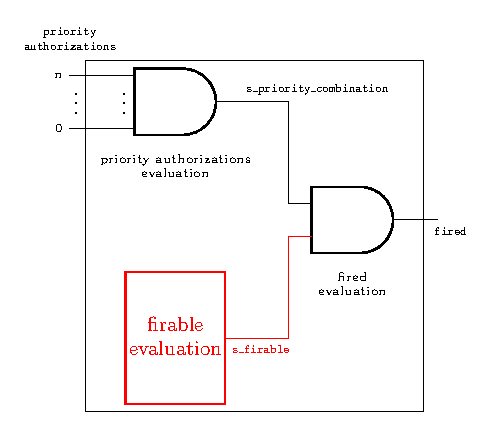
\includegraphics[keepaspectratio,width=.6\textwidth]{Figures/Proof/fired-port}
  \caption[The fired port of the transition design]{Wiring of the
    \texttt{fired} output port in the transition design architecture;
    on the left side is the input interface of the transition design;
    on the right side is the output interface of the transition
    design, with the \texttt{fired} port; in red are the parts of the
    architecture that depend on synchronous logic and in black are the
    parts that are purely combinational.}
  \label{fig:fired-port}
\end{figure}

In Figure~\ref{fig:fired-port}, the labels underneath the \emph{and}
logic ports and inside the block denote the names of the processes
defined in the transition design architecture as VHDL code. As a
matter of fact, Figure~\ref{fig:fired-port} is a transcription of the
code defining the transition design architecture. Therefore, by
looking at the VHDL code, we are able to determine the combinational
equation associated to the \texttt{fired} port. Considering a
transition component instance $id_t$ in a top-level design $d$; a
state $\sigma$ denotes the current stable state of $d$ (remember that
combinational equation hold when the signal values are stable); state
$\sigma(id_t)$ denotes the internal state of the transition component
instance $id_t$ at state $\sigma$; thus, the \texttt{fired} port
equation at $\sigma$ is:

\begin{equation}
  \label{eq:fired-port-comb-eq}
  \sigma(id_t)("fired")=\sigma(id_t)("s\_firable")~.~\sigma(id_t)("s\_priority\_combination")
\end{equation}

Equation~\eqref{eq:fired-port-comb-eq} states that the value of the
\texttt{fired} port is a simple ``and'' expression\footnote{To
  differentiate the formulas of the intuitionistic logic from the
  expressions of the boolean logic, we use (``$.$'', ``+'') to denote
  the \emph{and} and \emph{or} operators in boolean expressions, and
  ($\land$,$\lor$) to denote the conjunction and the disjunction in
  the intuitionistic formulas.} between the value of the internal
signal \texttt{s\_firable} and \texttt{s\_priority\_combination}.

\begin{remark}[Signals and combinational equations]
  \label{rmk:comb-eqs}
  In the proceeding of the proof, a lot of combinational equations are
  established (e.g, Equation~\eqref{eq:fired-port-comb-eq}). These
  equations link the value of a given signal to the value of other
  signals or expressions . All these equations are deduced by running
  the \hvhdl{} semantics rules on the internal behavior (i.e, the
  processes) of the transition and the place designs. A combinational
  equation is always the result of a signal assignment statement
  happening inside the statement body of a process. For instance, in
  the transition design, the \texttt{fired\_evaluation} process,
  presented in Listing~\ref{lst:fired-eval-ps}, assigns the
  \texttt{fired} output port.  Reasoning on the
  \texttt{fired\_evaluation} process statement body and on the
  \hvhdl{} semantics rules permits us to deduce
  Equation~\eqref{eq:fired-port-comb-eq}.

\begin{lstlisting}[language=VHDL,label={lst:fired-eval-ps},caption={The \texttt{fired\_evaluation} process in the transition design architecture; its body statement assigns the \texttt{fired} output port; symbol $\Leftarrow$ is the signal assignment operator}.]
fired_evaluation : process (s_firable, s_priority_combination)
begin
   fired <= s_firable and s_priority_combination;
end process fired_evaluation;
\end{lstlisting}

  Listing~\ref{lst:pauths-eval-ps} presents the
  \texttt{priority\_}\texttt{authorizations\_}\texttt{evaluation}
  process, responsible for the assignment of the
  \texttt{s\_priority\_combination} in the transition
  design. 

\begin{lstlisting}[language=VHDL,label={lst:pauths-eval-ps},caption={The \texttt{priority\_authorizations\_evaluation} process in the transition design's architecture. The local variable \texttt{v\_priority\_combination} accumulates the product of the \texttt{priority\_authorizations} input ports in the \texttt{for} loop; then the last statement assigns the value of \texttt{v\_priority\_combination} to the \texttt{s\_priority\_combination} internal signal.}]
priority_authorization_evaluation : process(priority_authorizations)
   variable v_priority_combination : std_logic;
begin
   v_priority_combination := '1';
    
   for i in 0 to input_arcs_number $-$ 1 loop
     v_priority_combination := v_priority_combination and priority_authorizations(i);
   end loop;
    
   s_priority_combination <= v_priority_combination; -- Assignment of the result
end process priority_authorization_evaluation;
\end{lstlisting}

  Equation~\eqref{eq:spc-comb-eq} gives the combinational equation
  deduced from the execution of the
  \texttt{priority\_}\texttt{authorizations\_}\texttt{evaluation}
  process for a given transition component instance $id_t$ in a
  top-level design $d$. State $\sigma$ denotes the current state of
  $d$, and $\sigma(id_t)$ denotes the internal state of $id_t$ at
  state $\sigma$. The elaborated design $\Delta$ is the elaborated
  version of design $d$, and $\Delta(id_t)$ is the elaborated version
  of $id_t$.
  
  \begin{equation}
    \label{eq:spc-comb-eq}
    \sigma(id_t)("spc")=\prod\limits_{i=0}^{\Delta(id_t)("input\_arcs\_number")-1}\sigma(id_t)("priority\_authorizations")[i]
  \end{equation}

  In Equation~\eqref{eq:spc-comb-eq}, ``spc'' is an alias\footnote{We
    will be using a lot of aliases for the names of signals in the
    proofs to come. Table~\ref{tab:consts-and-sigs-ref} gives the
    correspondence between signals and constants names and their
    aliases.} for the \texttt{s\_priority\_combination} signal.  The
  \texttt{for} loop of the
  \texttt{priority\_authorization\_evaluation} process has been
  converted into a product expression where the index $i$ follows the
  bounds of the loop. The \texttt{priority\_authorizations} signal is
  an input port of type \texttt{array}, thus we use the bracketed
  notation $a[i]$ to access the element of index $i$ in array
  $a$. Also, we know that \texttt{input\_arcs\_number} identifies a
  generic constant of the transition design, thus, we can retrieve its
  value in the elaborated design $\Delta(id_t)$.
  
  In the proofs laid out in Appendix~\ref{app:sem-preserv-proof} and
  in this chapter, we do not detail how the execution of processes's
  statement body permit to deduce combinational equations. We find
  that the proofs are easier to follow without entering in so much
  details. We let aside the task of proving that these equations hold
  until the time of the mechanization with the \coq{} proof
  assistant. For now, the reader can convince himself/herself that an
  equation holds by looking at the code of the place and the
  transition designs (see Appendix\todo{Add ref.}).
\end{remark}

Now that we know which combinational equation is attached to the value
of the output port \texttt{fired} for a given transition component
instance, we must relate this equation to the definition of the set of
fired transitions on the SITPN side. By definition of the set of fired
transitions, we know that $t\in{}Fired(s')$ is equivalent to
$t\in{}Firable(s')\land{}t\in{}Sens(s'.M-\sum\limits_{t_i\in{}Pr(t,s')}pre(t_i))$
where $Pr(t,s')=\{t'~\vert~t'\succ{}t\land{}t'\in{}Fired(s')\}$. By
definition of the \texttt{fired} port equation, we know that
$\sigma'(id_t)("fired")=\sigma'(id_t)("s\_firable")~.~\sigma'(id_t)("s\_priority\_combination")$.
Using these definitions to rewrite the terms of the current goal, the
new goal to prove is:

\begin{frameb}
  $t\in{}Firable(s')\land{}t\in{}Sens(s'.M-\sum\limits_{t_i\in{}Pr(t,s')}pre(t_i))\Leftrightarrow$\\
  $\sigma'(id_t)("s\_firable")~.~\sigma'(id_t)("s\_priority\_combination")=\mathtt{true}$
\end{frameb}

Thanks to Lemma~\ref{lem:fe-equal-firable}, we know that
$t\in{}Firable(s')$ iff
$\sigma'(id_t)("s\_firable")=\mathtt{true}$. Then, we can get rid of
these two terms in the current goal; then, what is left to prove is:

\begin{frameb}
  $t\in{}Sens(s'.M-\sum\limits_{t_i\in{}Pr(t,s')}pre(t_i))\Leftrightarrow$\\
  $\big(\prod\limits_{i=0}^{\Delta(id_t)("input\_arcs\_number")-1}\sigma'(id_t)("priority\_authorizations")[i]\big)=\mathtt{true}$
\end{frameb}

Then, the proof is in two parts:

\begin{enumerate}
\item Assuming
  $t\in{}Sens(s'.M-\sum\limits_{t_i\in{}Pr(t,s')}pre(t_i))$, let us
  show that\\
  \fbox{$\big(\prod\limits_{i=0}^{\Delta(id_t)("ian")-1}\sigma'(id_t)("pauths")[i]\big)=\mathtt{true}$.}
\item Assuming
  $\big(\prod\limits_{i=0}^{\Delta(id_t)("ian")-1}\sigma'(id_t)("pauths")[i]\big)=\mathtt{true}$,
  let us show that\\
  \fbox{$t\in{}Sens(s'.M-\sum\limits_{t_i\in{}Pr(t,s')}pre(t_i))$.}
\end{enumerate}

\noindent{}Let us prove the first point. Assuming that
$t\in{}Sens(s'.M-\sum\limits_{t_i\in{}Pr(t,s')}pre(t_i))$, let us
show\\
\fbox{$\big(\prod\limits_{i=0}^{\Delta(id_t)("ian")-1}\sigma'(id_t)("pauths")[i]\big)=\mathtt{true}$.}\\

\noindent{}To prove the current goal, we can equivalently show that:\\
\fbox{$\forall{}i\in[0,\Delta(id_t)("ian")-1],~\sigma'(id_t)("pauths")[i]=\mathtt{true}$.}

\noindent{}For a given $i\in[0,\Delta(id_t)("ian")-1]$, let us show
that \fbox{$\sigma'(id_t)("pauths")[i]=\mathtt{true}$.} As shown in
Figure~\ref{fig:fired-port}, the signal
\texttt{priority\_authorizations} is an input port of the transition
design. Therefore, to know what is the value of the element $i$-th
element of port \texttt{priority\_authorizations} at state
$\sigma'(id_t)$, we must know how the
\texttt{priority\_authorizations} port is connected in the top-level
design. Basing ourselves on the transformation function, the
connection of the \texttt{priority\_authorizations} port for the
transition component instance $id_t$ depends on the set of input
places of the transition $t$. If the set of input places of $t$ is
empty, then, all elements of the \texttt{priority\_authorizations}
port are connected to the constant \texttt{true}, and proving the goal
is trivial. If the set of input places of $t$ is not empty, then, the
connection of the $i$-th element of the
\texttt{priority\_authorizations} port reflects the connection of some
place $p$ to the transition $t$ by an input arc. Then, we must reason
on the nature of the input arc connecting $p$ to $t$. The interested
case happens when $p$ and $t$ are connected by a \texttt{basic} arc,
and when the conflicts in the output transitions of $p$ are handled by
the priority relation.

%%%%%%%%%%%%%%%%%%%%%%%%%%%%%%%%%%%%%%%%%%%%%%%%%%%%%%%%
%%%%%%%%%% FALLING EDGE NOT EQUAL FIRED LEMMA %%%%%%%%%%
%%%%%%%%%%%%%%%%%%%%%%%%%%%%%%%%%%%%%%%%%%%%%%%%%%%%%%%%

\begin{lemma}[Falling Edge Equal Not Fired]
  \label{lem:fe-equal-not-fired}
  \fehyps{} then $\forall{}t,id_t~s.t.~\gamma(t)=id_t,$
  $~t\notin{}Fired(s')\Leftrightarrow\sigma'_t("fired")=\mathtt{false}$.
\end{lemma}


\begin{proof}
  Proving the above lemma is trivial by appealing to
  Lemma~\nameref{lem:fe-equal-fired} and by reasoning on
  contrapositives.
\end{proof}

%%%%%%%%%%%%%%%%%%%%%%%%%%%%%%%%%%%%%%%%%%%%%%%%%%%%%%%%
%%%%%%%%%% FALLING EDGE EQUAL FIRED SET LEMMA %%%%%%%%%%
%%%%%%%%%%%%%%%%%%%%%%%%%%%%%%%%%%%%%%%%%%%%%%%%%%%%%%%%


\begin{lemma}[Falling Edge Equal Fired Set]
  \label{lem:fe-equal-fset}
  \fehyps{} then
  $\forall{}t\in{}T,~id_t\in{}Comps(\Delta)~s.t.~\gamma(t)=id_t$,
  $\forall{}fset\subseteq{}T,~s.t.~IsFiredSet(s',fset),~t\in{}fset\Leftrightarrow\sigma'(id_t)("fired")=true$.
\end{lemma}

\begin{niproof}
  Given a $t\in{}T$, and $id_t\in{}Comps(\Delta)$, and a
  $fset\subseteq{}T$ s.t. $IsFiredSet(s',fset)$, let us show
  \fbox{$t\in{}fset\Leftrightarrow\sigma'(id_t)("fired")=true$.}\\

  By definition of $IsFiredSet(s',fset)$, we have
  $IsFiredSetAux(s',\emptyset,T,fset)$.

  Then, we can appeal to Lemma~\nameref{lem:fe-equal-fset-aux} to
  solve the goal, but first we must prove the following \emph{extra
    hypothesis} (i.e, one of the premise of
  Lemma~\nameref{lem:fe-equal-fset-aux}):

  \fbox{\parbox{\lwidth}{$\forall{}t'\in{}T,id_{t'}\in{}Comps(\Delta)$
      s.t. $\gamma(t')=id_{t'},$\\
      $(t'\in{}\emptyset\Rightarrow\sigma'(id_{t'})("fired")=\mathtt{true})$
      $\land$
      $(\sigma'(id_{t'})("fired")=\mathtt{true}\Rightarrow{}t'\in{}\emptyset~\lor~{}t'\in{}T)$.}}\\

  Given a $t'\in{}T$ and an $id_{t'}\in{}Comps(\Delta)$
  s.t. $\gamma(t')=id_{t'}$, there are two points to prove:
  \begin{enumerate}
  \item
    \fbox{$t'\in{}\emptyset\Rightarrow\sigma'(id_{t'})("fired")=\mathtt{true}$}
  \item
    \fbox{$\sigma'(id_{t'})("fired")=\mathtt{true}\Rightarrow{}t'\in{}\emptyset~\lor~{}t'\in{}T$}
  \end{enumerate}

  Let us show these two points:
  \begin{enumerate}
  \item Assuming $t'\in{}\emptyset$, let us show
    \fbox{$\sigma'(id_{t'})("fired")=\mathtt{true}$.}

    \qedbox{$t'\in{}\emptyset$ is a contradiction.}
  \item Assuming $\sigma'(id_{t'})("fired")=\mathtt{true}$, let us
    show \fbox{$t'\in{}\emptyset~\lor~{}t'\in{}T$.}

    By definition, \qedbox{$t'\in{}T$.}
  \end{enumerate}
  
\end{niproof}

%%%%%%%%%%%%%%%%%%%%%%%%%%%%%%%%%%%%%%%%%%%%%%%%%%%%%%%%%%%%
%%%%%%%%%% FALLING EDGE EQUAL FIRED SET AUX LEMMA %%%%%%%%%%
%%%%%%%%%%%%%%%%%%%%%%%%%%%%%%%%%%%%%%%%%%%%%%%%%%%%%%%%%%%%

\begin{lemma}[Falling Edge Equal Fired Set Aux]
  \label{lem:fe-equal-fset-aux}
  \fehyps{} then
  $\forall{}t\in{}T,id_t\in{}Comps(\Delta)~s.t.~\gamma(t)=id_t$,
  $\forall{}fired\subseteq{}T,~T_s\subseteq{}T,~fset\subseteq{}T,$
  assume that:
  \begin{itemize}
  \item $IsFiredSetAux(s',fired,T_s,fset)$
  \item EH (Extra. Hypothesis):\\
    $\forall{}t'\in{}T,~id_{t'}\in{}Comps(\Delta)$
    s.t. $\gamma(t')=id_{t'}$,\\
    $(t'\in{}fired\Rightarrow\sigma'(id_{t'})("fired")=\mathtt{true})$
    $\land$
    $(\sigma'(id_{t'})("fired")=\mathtt{true}\Rightarrow{}t'\in{}fired~\lor~{}t'\in{}T_s)$.
  \end{itemize}
  then
  $t\in{}fset\Leftrightarrow\sigma'(id_t)("fired")=\mathtt{true}$.
\end{lemma}

\begin{niproof}
  Given a $t\in{}T$, an $id_t\in{}Comps(\Delta)$, a
  $fired,T_s,fset\subseteq{}T$, and assuming\\
  $IsFiredSetAux(s',fired,T_s,fset)$ and EH, let us show
  \fbox{$t\in{}fset\Leftrightarrow\sigma'(id_t)("fired")=\mathtt{true}$.}

  Let us reason by induction on $IsFiredSetAux(s',fired,T_s,fset)$.

  \begin{itemize}
  \item \textbf{BASE CASE}:
    \fbox{$t\in{}fired\Leftrightarrow\sigma'(id_t)("fired")=\mathtt{true}$.}

    In that case, $fired=fset$ and $T_s=\emptyset$, EH looks like
    this:

    \parbox{\lwidth}{$\forall{}t'\in{}T,~id_{t'}\in{}Comps(\Delta)$
      s.t. $\gamma(t')=id_{t'}$,\\
      $(t'\in{}fired\Rightarrow\sigma'(id_{t'})("fired")=\mathtt{true})$
      $\land$
      $(\sigma'(id_{t'})("fired")=\mathtt{true}\Rightarrow{}t'\in{}fired~\lor~{}t'\in{}\emptyset)$.}

    From EH, we can deduce
    \qedbox{$t\in{}fired\Leftrightarrow\sigma'(id_t)("fired")=\mathtt{true}$.}
    
  \item \textbf{INDUCTION CASE}:
    \fbox{$t\in{}fset\Leftrightarrow\sigma'(id_t)("fired")=\mathtt{true}$.}

    In that case, we have:
    \begin{itemize}
    \item $IsTopPrioritySet(T_s,tp)$
    \item $ElectFired(s',fired,tp,fired')$
    \item $FiredAux(s',fired',T_s\setminus{}tp,fset)$
    \end{itemize}

    \begin{ih}
      $\big(\forall{}t'\in{}T,id_{t'}\in{}Comps(\Delta)~s.t.~\gamma(t')=id_{t'},$\\
      $(t'\in{}fired'\Rightarrow\sigma'(id_{t'})("fired")=\mathtt{true})$
      $\land(\sigma'(id_{t'})("fired")=\mathtt{true}\Rightarrow{}t'\in{}fired'~\lor~{}t'\in{}T_s\setminus{}tp)\big)\Rightarrow$\\
      $t\in{}fset\Leftrightarrow\sigma'_t("fired")=true$.
    \end{ih}
    
    Applying the induction hypothesis, then, the new goal is:
    \begin{frameb}
      $\forall{}t'\in{}T,id_{t'}\in{}Comps(\Delta)~s.t.~\gamma(t')=id_{t'},$\\
      $(t'\in{}fired'\Rightarrow\sigma'(id_{t'})("fired")=\mathtt{true})$\\
      $\land(\sigma'(id_{t'})("fired")=\mathtt{true}\Rightarrow{}t'\in{}fired'~\lor~{}t'\in{}T_s\setminus{}tp)$
    \end{frameb}
    
    Apply Lemma~\nameref{lem:elect-fired-equal-fired} to solve the goal.
    
  \end{itemize}
  
\end{niproof}

%%%%%%%%%%%%%%%%%%%%%%%%%%%%%%%%%%%%%%%%%%%%%
%%%%%%%%%% ELECT FIRED EQUAL FIRED %%%%%%%%%%
%%%%%%%%%%%%%%%%%%%%%%%%%%%%%%%%%%%%%%%%%%%%%

\begin{lemma}[Elect Fired Equal Fired]
  \label{lem:elect-fired-equal-fired}
  \fehyps{} then
  $\forall{}fired,fired',T_s,tp,~fset\subseteq{}T,$
  assume that:
  \begin{itemize}
  \item $IsTopPrioritySet(T_s,tp)$
  \item $ElectFired(s',fired,tp,fired')$
  \item $FiredAux(s',fired',T_s\setminus{}tp,fset)$
  \item EH (Extra. Hypothesis):\\
    $\forall{}t'\in{}T,id_{t'}\in{}Comps(\Delta)~s.t.~\gamma(t')=id_{t'}$,\\
    $(t'\in{}fired\Rightarrow\sigma'(id_{t'})("fired")=\mathtt{true})$
    $\land$
    $(\sigma'(id_{t'})("fired")=\mathtt{true}\Rightarrow{}t'\in{}fired~\lor~{}t'\in{}T_s)$
  \end{itemize}
  then $\forall{}t\in{}T,id_t\in{}Comps(\Delta)$
  s.t. $\gamma(t)=id_t$,\\
  $\big(t\in{}fired'\Rightarrow\sigma'(id_t)("fired")=\mathtt{true}\big)$
  $\land\big(\sigma'(id_t)("fired")=\mathtt{true}\Rightarrow{}t\in{}fired'\lor{}t\in{}T_s\setminus{}tp\big)$.
\end{lemma}

\begin{niproof}
  Given a $t\in{}T$ and an $id_t\in{}Comps(\Delta)$
  s.t. $\gamma(t)=id_t$, let us show\\
  \fbox{$\big(t\in{}fired'\Rightarrow\sigma'(id_t)("fired")=\mathtt{true}\big)$
    $\land\big(\sigma'(id_t)("fired")=\mathtt{true}\Rightarrow{}t\in{}fired'\lor{}t\in{}T_s\setminus{}tp\big)$.}\\
  
  Let us reason by induction on $ElectFired(s',fired,tp,fired')$;
  there are three cases:

  \begin{enumerate}
  \item \textbf{BASE CASE}: $tp=\emptyset$ and $fired=fired'$.
  \item \textbf{INDUCTIVE CASE}: $tp=\{t_0\}\cup{}tp_0$ and $t_0$ is
    elected to be fired.
  \item \textbf{INDUCTIVE CASE}: $tp=\{t_0\}\cup{}tp_0$ and $t_0$ is
    not elected to be fired.
  \end{enumerate}

  Let us prove the goal in these three contexts:

  \begin{enumerate}
  \item \textbf{BASE CASE}:
    
    \fbox{\parbox{\lwidth}{$\big(t\in{}fired\Rightarrow\sigma'(id_t)("fired")=\mathtt{true}\big)$
        $\land\big(\sigma'(id_t)("fired")=\mathtt{true}\Rightarrow{}t\in{}fired\lor{}t\in{}T_s\big)$.}}
    
    \qedbox{Apply EH to solve the goal.}
    
  \item \textbf{INDUCTIVE CASE}: $tp=\{t_0\}\cup{}tp_0$ and $t_0$ is
    elected to be fired.

    In that case, we have:
    \begin{itemize}
    \item
      $IsTopPrioritySet(T_s,\{t_0\}\cup{}tp_0)$
    \item $ElectFired(s',fired\cup\{t_0\},tp_0,fired')$
    \item
      $IsFiredSetAux(s',fired',T_s\setminus\{t_0\}\cup{}tp_0,fset)$
    \item $t_0\in{}Firable(s')$
    \item
      $t_0\in{}Sens(s'.M-\sum\limits_{t_i\in{}Pr(t,fired)}pre(t_i))$
      where $Pr(t,fired)=\{t'~\vert~t'\succ{}t\land{}t'\in{}fired\}$
    \item EH: $\forall{}t'\in{}T,~id_{t'}\in{}Comps(\Delta)$
      s.t. $\gamma(t')=id_{t'}$,\\
      $(t'\in{}fired\Rightarrow\sigma'(id_{t'})("f")=\mathtt{true})$
      $\land$
      $(\sigma'(id_{t'})("f")=\mathtt{true}\Rightarrow{}t'\in{}fired~\lor~{}t'\in{}T_s)$
    \end{itemize}

    \begin{ih}
      $\forall{}T'_s\subseteq{}T,~$\\
      $IsTopPrioritySet(T'_s,tp_0)\Rightarrow$\\
      $IsFiredSetAux(s',fired',T'_s\setminus{}tp_0,fset)\Rightarrow$\\
      $\big(\forall{}t'\in{}T,id_{t'}\in{}Comps(\Delta)$ s.t. $\gamma(t')=id_{t'}$,\\
      $(t'\in{}fired\cup\{t_0\}\Rightarrow\sigma'_{t'}("f")=\mathtt{true})$
      $\land$
      $(\sigma'(id_{t'})("f")=\mathtt{true}\Rightarrow{}t'\in{}fired\cup\{t_0\}~\lor~{}t'\in{}T'_s)\big)\Rightarrow$\\
      $\forall{}t\in{}T,~id_t\in{}Comps(\Delta)$ s.t. $\gamma(t)=id_t$,\\
      $~\big(t\in{}fired'\Rightarrow\sigma'(id_t)("f")=\mathtt{true}\big)$
      $\land$
      $\big(\sigma'(id_t)("f")=\mathtt{true}\Rightarrow{}t\in{}fired'\lor{}t\in{}T'_s\setminus{}tp_0\big)$
    \end{ih}
    
    \begin{frameb}
      $\forall{}t\in{}T,~id_t\in{}Comps(\Delta)$
      s.t. $\gamma(t)=id_t$,\\
      $~\big(t\in{}fired'\Rightarrow\sigma'_t("f")=\mathtt{true}\big)$
      $\land$
      $\big(\sigma'_t("f")=\mathtt{true}\Rightarrow{}t\in{}fired'\lor{}t\in{}T_s\setminus{}\{t_0\}\cup{}tp_0\big)$
    \end{frameb}
    
    To solve the goal, we can apply the induction hypothesis with
    $T'_s=T_s\setminus\{t_0\}$; then, there are three points to prove:
    \begin{enumerate}
    \item
      \fbox{$IsTopPrioritySet(T_s\setminus\{t_0\},tp_0)$}
    \item
      \fbox{$IsFiredSetAux(s',fired',(T_s\setminus\{t_0\})\setminus{}tp_0,fset)$}
    \item \fbox{\parbox{\lwidth}{$\forall{}t'\in{}T,id_{t'}\in{}Comps(\Delta)$ s.t. $\gamma(t')=id_{t'}$,\\
          $(t'\in{}fired\cup\{t_0\}\Rightarrow\sigma'_{t'}("f")=\mathtt{true})$
          $\land$
          $(\sigma'(id_{t'})("f")=\mathtt{true}\Rightarrow{}t'\in{}fired\cup\{t_0\}~\lor~{}t'\in{}T_s\setminus\{t_0\})$}}
    \end{enumerate}

    Let us prove these three points:
    \begin{enumerate}
    \item
      \fbox{$IsTopPrioritySet(T_s\setminus\{t_0\},tp_0)$}
      \begin{todobox}
        Not provable yet.
      \end{todobox}
    \item
      \fbox{$IsFiredSetAux(s',fired',(T_s\setminus\{t_0\})\setminus{}tp_0,fset)$}.
      
      We know that
      $(T_s\setminus\{t_0\})\setminus{}tp_0=T_s\setminus{}(\{t_0\}\cup{}tp_0)$,
      and thus\\
      \qedbox{$IsFiredSetAux(s',fired',T_s\setminus{}(\{t_0\}\cup{}tp_0),fset)$
        is an assumption.}
      
    \item \fbox{\parbox{\lwidth}{$\forall{}t'\in{}T,id_{t'}\in{}Comps(\Delta)$ s.t. $\gamma(t')=id_{t'}$,\\
          $(t'\in{}fired\cup\{t_0\}\Rightarrow\sigma'(id_{t'})("f")=\mathtt{true})$
          $\land$
          $(\sigma'(id_{t'})("f")=\mathtt{true}\Rightarrow{}t'\in{}fired\cup\{t_0\}~\lor~{}t'\in{}T_s\setminus\{t_0\})$}}\\

      Given a $t'\in{}T$ and an $id_{t'}\in{}Comps(\Delta)$
      s.t. $\gamma(t')=id_{t'}$, let us show\\
      \fbox{\parbox{\lwidth}{$(t'\in{}fired\cup\{t_0\}\Rightarrow\sigma'(id_{t'})("f")=\mathtt{true})$\\
          $\land$
          $(\sigma'(id_{t'})("f")=\mathtt{true}\Rightarrow{}t'\in{}fired\cup\{t_0\}~\lor~{}t'\in{}T_s\setminus\{t_0\})$.}}
      
      The proof is in two parts.
      
      \begin{enumerate}
      \item Assuming that $t'\in{}fired\cup\{t_0\}$, let us show
        \fbox{$\sigma'(id_{t'})("f")=\mathtt{true}$.}

        Case analysis on $t'\in{}fired\cup\{t_0\}$; there are two cases:
        \begin{itemize}
        \item $t'\in{}fired$
        \item $t'=t_0$
        \end{itemize}

        Let us prove the goal in these two contexts.
        
        \begin{itemize}
        \item \textbf{CASE} $t'\in{}fired$: Thanks to EH, we can
          deduce \qedbox{$\sigma'_{t'}("f")=\mathtt{true}$.}
          
        \item \textbf{CASE} $t'=t_0$:
          
          By definition of $id_{t'}$, there exist a $gm_{t'}$,
          $ipm_{t'}$, $opm_{t'}$ s.t.
          $\mathtt{comp}(id_{t'},"transition",$ $gm_{t'},$ $ipm_{t'}$,
          $opm_{t'})\in{}d.cs$.

          By property of the stabilize relation and
          $\mathtt{comp}(id_{t'},"transition",$ $gm_{t'},$ $ipm_{t'}$,
          $opm_{t'})\in{}d.cs$:
          \begin{equation}
            \label{eq:frd-eq-frd}
            \sigma(id_{t'})("f")=\sigma(id_{t'})("sfa")~.~\sigma(id_{t'})("spc")
          \end{equation}

          Rewriting the goal with \eqref{eq:frd-eq-frd}:
          \fbox{$\sigma(id_{t'})("sfa")~.~\sigma(id_{t'})("spc")=\mathtt{true}$.}
          
          Then, we can show that: 
          \begin{itemize}
          \item $\sigma(id_{t'})("sfa")=\mathtt{true}$ by applying
            Lemma~\nameref{lem:fe-equal-firable}
          \item $\sigma(id_{t'})("spc")=\mathtt{true}$ by applying
            Lemma~\nameref{lem:stab-compute-pcomb}.
          \end{itemize}
        \end{itemize}
        
      \item Assuming that $\sigma'(id_{t'})("f")=\mathtt{true}$, let
        us show
        \fbox{$t'\in{}fired\cup\{t_0\}~\lor~{}t'\in{}T_s\setminus{}\{t_0\}$.}

        From $\sigma'(id_{t'})("f")=\mathtt{true}$ and EH, we can
        deduce that $t'\in{}fired\lor{}t'\in{}T_s$.

        Case analysis on $t'\in{}fired\lor{}t'\in{}T_s$.
        
        \begin{itemize}
        \item \textbf{CASE} $t'\in{}fired$: then, it is trivial to
          show \qedbox{$t'\in{}fired\cup\{t_0\}$.}
        \item \textbf{CASE} $t'\in{}T_s$: We know that $t_0\in{}T_s$.
          Therefore, either \qedbox{$t'\in{}T_s\setminus{}\{t_0\}$},
          or $t'=t_0$, and then, \qedbox{$t'\in{}fired\cup\{t_0\}$.}
        \end{itemize}
      \end{enumerate}
    \end{enumerate}
  \end{enumerate}

  \begin{enumerate}[resume]
  \item \textbf{INDUCTIVE CASE}: $tp=\{t_0\}\cup{}tp_0$ and $t_0$ is
    not elected to be fired.
    \begin{itemize}
    \item $IsTopPrioritySet(T_s,\{t_0\}\cup{}tp_0)$
    \item $ElectFired(s',fired,tp_0,fired')$
    \item $IsFiredSetAux(s',fired',T_s\setminus\{t_0\}\cup{}tp_0,fset)$
    \item $\neg\big(t_0\in{}Firable(s')\land{}t_0\in{}Sens(s'.M-\sum\limits_{t_i\in{}Pr(t,fired)}pre(t_i))\big)$
    \item EH:\\
      $\forall{}t'\in{}T,id_{t'}\in{}Comps(\Delta)$ s.t. $\gamma(t')=id_{t'}$,\\
      $(t'\in{}fired\Rightarrow\sigma'(id_{t'})("f")=\mathtt{true})$
      $\land$
      $(\sigma'(id_{t'})("f")=\mathtt{true}\Rightarrow{}t'\in{}fired~\lor~{}t'\in{}T_s)$
    \end{itemize}

    \begin{ih}
      $\forall{}T'_s\subseteq{}T,~$\\
      $IsTopPrioritySet(T'_s,tp_0)\Rightarrow$\\
      $IsFiredSetAux(s',fired',T'_s\setminus{}tp_0,fset)\Rightarrow$\\
      $\big(\forall{}t'\in{}T,id_{t'}\in{}Comps(\Delta)$
      s.t. $\gamma(t')=id_{t'},$\\
      $(t'\in{}fired\Rightarrow\sigma'(id_{t'})("f")=\mathtt{true})$
      $\land$
      $(\sigma'(id_{t'})("f")=\mathtt{true}\Rightarrow{}t'\in{}fired~\lor~{}t'\in{}T'_s)\big)\Rightarrow$\\
      $\forall{}t\in{}T,id_t\in{}Comps(\Delta)$ s.t. $\gamma(t)=id_t$,\\
      $~\big(t\in{}fired'\Rightarrow\sigma'(id_t)("f")=\mathtt{true}\big)$
      $\land$
      $\big(\sigma'(id_t)("f")=\mathtt{true}\Rightarrow{}t\in{}fired'\lor{}t\in{}T'_s\setminus{}tp_0\big)$
    \end{ih}
    
    \fbox{\parbox{\lwidth}{$\forall{}t\in{}T,id_t\in{}Comps(\Delta)$ s.t. $\gamma(t)=id_t$,\\
        $~\big(t\in{}fired'\Rightarrow\sigma'(id_t)("f")=\mathtt{true}\big)$
        $\land$
        $\big(\sigma'(id_t)("f")=\mathtt{true}\Rightarrow{}t\in{}fired'\lor{}t\in{}T_s\setminus{}\{t_0\}\cup{}tp_0\big)$.}}
    
    Then, we can apply the induction hypothesis with
    $T'_s=T_s\setminus\{t_0\}$, then, there are three points to prove:

    \begin{enumerate}
    \item
      \fbox{$IsTopPrioritySet(T_s\setminus\{t_0\},tp_0)$}
    \item
      \fbox{$IsFiredSetAux(s',fired',(T_s\setminus\{t_0\})\setminus{}tp_0,fset)$}
    \item \fbox{\parbox{\lwidth}{$\forall{}t'\in{}T,id_{t'}\in{}Comps(\Delta)$
          s.t. $\gamma(t')=id_{t'}$,\\
          $(t'\in{}fired\Rightarrow\sigma'(id_{t'})("f")=\mathtt{true})$
          $\land$
          $(\sigma'(id_{t'})("f")=\mathtt{true}\Rightarrow{}t'\in{}fired~\lor~{}t'\in{}T_s\setminus\{t_0\})$}}
    \end{enumerate}

    Let us prove these three points:

    \begin{enumerate}
    \item \fbox{$IsTopPrioritySet(T_s\setminus\{t_0\},tp_0)$}
      \begin{todobox}
        Not provable yet.
      \end{todobox}
    \item
      \fbox{$IsFiredSetAux(s',fired',(T_s\setminus\{t_0\})\setminus{}tp_0,fset)$}

      We know that
      $(T_s\setminus\{t_0\})\setminus{}tp_0=T_s\setminus{}(\{t_0\}\cup{}tp_0)$,
      and thus\\
      \qedbox{$IsFiredSetAux(s',fired',T_s\setminus{}(\{t_0\}\cup{}tp_0),fset)$
        is an assumption.}
      
    \item
      \fbox{\parbox{\lwidth}{$\forall{}t'\in{}T,id_{t'}\in{}Comps(\Delta)$
          s.t. $\gamma(t')=id_{t'}$,\\
          $(t'\in{}fired\Rightarrow\sigma'(id_{t'})("f")=\mathtt{true})$
          $\land$
          $(\sigma'(id_{t'})("f")=\mathtt{true}\Rightarrow{}t'\in{}fired~\lor~{}t'\in{}T_s\setminus\{t_0\})$}}

      Given a $t'\in{}T$ and an $id_{t'}\in{}Comps(\Delta)$
      s.t. $\gamma(t')=id_{t'}$, let us show

      \begin{frameb}
        $(t'\in{}fired\Rightarrow\sigma'(id_{t'})("f")=\mathtt{true})$
        $\land$
        $(\sigma'(id_{t'})("f")=\mathtt{true}\Rightarrow{}t'\in{}fired~\lor~{}t'\in{}T_s\setminus\{t_0\})$
      \end{frameb}

      The proof is in two parts:
      
      \begin{enumerate}
      \item Assuming that $t'\in{}fired$, let us show
        \fbox{$\sigma'(id_{t'})("f")=\mathtt{true}$.}

        From $t'\in{}fired$ and EH,
        \qedbox{$\sigma'(id_{t'})("f")=\mathtt{true}$.}
        
      \item Assuming that $\sigma'(id_{t'})("f")=\mathtt{true}$, let
        us show
        \fbox{$t'\in{}fired~\lor~{}t'\in{}T_s\setminus{}\{t_0\}$.}

        Thanks to $\sigma'(id_{t'})("f")=\mathtt{true}$ and EH, we
        know that: $t'\in{}fired\lor{}t'\in{}T_s$.

        Case analysis on $t'\in{}fired\lor{}t'\in{}T_s$; there are two
        cases:
        \begin{itemize}
        \item \textbf{CASE} \qedbox{$t'\in{}fired$.}
        \item \textbf{CASE} $t'\in{}T_s$:

          From $IsTopPrioritySet(T_s,\{t_0\}\cup{}tp_0)$, we can
          deduce that $t_0\in{}T_s$. Therefore, either
          \qedbox{$t'\in{}T_s\setminus{}\{t_0\}$} or $t'=t_0$.

          In the case where $t'=t_0$, we need to show a contradiction by proving\\
          $t'\in{}Firable(s')$ and
          $t'\in{}Sens(s'.M-\sum\limits_{t_i\in{}Pr(t,fired)}pre(t_i))$
          based on $\sigma'(id_{t'})("f")=\mathtt{true}$.

          By definition of $id_{t'}$, there exist a $gm_{t'}$,
          $ipm_{t'}$, $opm_{t'}$ s.t.
          $\mathtt{comp}(id_{t'},"transition",$ $gm_{t'},$ $ipm_{t'}$,
          $opm_{t'})\in{}d.cs$.

          By property of the stabilize relation and
          $\mathtt{comp}(id_{t'},$ $"transition",$ $gm_{t'},$
          $ipm_{t'}$, $opm_{t'})\in{}d.cs$:
          \begin{equation}
            \label{eq:frd-eq-frd-true}
            \sigma(id_{t'})("f")=\sigma(id_{t'})("sfa")~.~\sigma(id_{t'})("spc")=\mathtt{true}
          \end{equation}

          From $\sigma(id_{t'})("sfa")=\mathtt{true}$, and appealing
          to Lemma~\nameref{lem:fe-equal-firable}, we can deduce
          $t'\in{}Firable(s')$.

          From $\sigma(id_{t'})("spc")=\mathtt{true}$, and appealing
          to Lemma~\nameref{lem:stab-compute-pcomb}, we can deduce
          $t'\in{}Sens(s'.M-\sum\limits_{t_i\in{}Pr(t,fired)}$ $pre(t_i))$.

          Then, as $t'=t_0$,
          $\neg\big(t_0\in{}Firable(s')\land{}t_0\in{}Sens(s'.M-\sum\limits_{t_i\in{}Pr(t,fired)}pre(t_i))\big)$
          is a \qedbox{contradiction.}
        \end{itemize}
      \end{enumerate}      
    \end{enumerate}
  \end{enumerate}
  
\end{niproof}

%%%%%%%%%%%%%%%%%%%%%%%%%%%%%%%%%%%%%%%%%%%%%%%%%%%%%%%%%%%%%%%%%%%%%%%%%%%%%%%
%%%%%%%%%% STABILIZE COMPUTE PRIORITY COMBINATION AFTER FALLING EDGE %%%%%%%%%%
%%%%%%%%%%%%%%%%%%%%%%%%%%%%%%%%%%%%%%%%%%%%%%%%%%%%%%%%%%%%%%%%%%%%%%%%%%%%%%%

\begin{lemma}[Stabilize Compute Priority Combination After Falling Edge]
  \label{lem:stab-compute-pcomb}
  \fehyps{} then
  $\forall{}t\in{}T,id_t\in{}Comps(\Delta)$ s.t. $\gamma(t)=id_t$,\\
  $\forall{}fired,fired',~T_s,~tp,~fset\subseteq{}T$ assume that:
  \begin{itemize}
  \item $IsTopPrioritySet(T_s,\{t\}\cup{}tp)$
  \item $ElectFired(s',fired,tp,fired')$
  \item $FiredAux(s',fired',T_s\setminus{}\{t\}\cup{}tp,fset)$
  \item EH: $\forall{}t'\in{}T,id_{t'}\in{}Comps(\Delta)$
    s.t. $\gamma(t')=id_{t'}$,\\
    $(t'\in{}fired\Rightarrow\sigma'(id_{t'})("f")=\mathtt{true})$
    $\land$
    $(\sigma'(id_{t'})("f")=\mathtt{true}\Rightarrow{}t'\in{}fired~\lor~{}t'\in{}T_s)$.
  \item $t\in{}Firable(s')$
  \end{itemize}
  then
  $t\in{}Sens(s'.M-\sum\limits_{t_i\in{}Pr(t,fired)}pre(t_i))\Leftrightarrow\sigma'(id_t)("spc")=\mathtt{true}$
\end{lemma}

\begin{niproof}

  Given a $t\in{}T$ and an $id_t\in{}Comps(\Delta)$
  s.t. $\gamma(t)=id_t$, a $fired$, $fired'$, $T_s$, $tp$,
  $fset\subseteq{}T$ and assuming all the above hypotheses, let us
  show\\
  \fbox{$t\in{}Sens(s'.M-\sum\limits_{t_i\in{}Pr(t,fired)}pre(t_i))\Leftrightarrow\sigma'(id_t)("spc")=\mathtt{true}$.}\\

  \exT{}
  
  By property of the stabilize relation and \InCsCompT:  
  \begin{equation}
    \sigma'(id_t)("spc")=\prod\limits_{i=0}^{\Delta(id_t)("ian")-1}\sigma'(id_t)("pauths")[i]\label{eq:frd-eq-spc-prod-pauths}
  \end{equation}

  Rewriting the goal with \eqref{eq:frd-eq-spc-prod-pauths}:
  
  \fbox{$t\in{}Sens(s'.M-\sum\limits_{t_i\in{}Pr(t,fired)}pre(t_i))\Leftrightarrow\prod\limits_{i=0}^{\Delta(id_t)("ian")-1}\sigma'(id_t)("pauths")[i]=\mathtt{true}$.}\\
  
  Then, the proof is in two parts:
  \begin{enumerate}
  \item
    $t\in{}Sens(s'.M-\sum\limits_{t_i\in{}Pr(t,fired)}pre(t_i))\Rightarrow\prod\limits_{i=0}^{\Delta(id_t)("ian")-1}\sigma'(id_t)("pauths")[i]=\mathtt{true}$
  \item
    $\prod\limits_{i=0}^{\Delta(id_t)("ian")-1}\sigma'(id_t)("pauths")[i]=\mathtt{true}\Rightarrow{}t\in{}Sens(s'.M-\sum\limits_{t_i\in{}Pr(t,fired)}pre(t_i))$
  \end{enumerate}

  Let us prove both sides of the equivalence:
  \begin{enumerate}
  \item\label{item:stab-comp-spc-fst-case}
    Assuming that
    $t\in{}Sens(s'.M-\sum\limits_{t_i\in{}Pr(t,fired)}pre(t_i))$, let
    us
    show\\
    \fbox{$\prod\limits_{i=0}^{\Delta(id_t)("ian")-1}\sigma'(id_t)("pauths")[i]=\mathtt{true}$.}

    Let us perform case analysis on $input(t)$; there are 2 cases:
    \begin{itemize}
    \item \textbf{CASE} $input(t)=\emptyset$:

      By construction,
      ${<}\mathtt{input\_arcs\_number\Rightarrow}{}1{>}\in{}gm_t$ and\\
      ${<}\mathtt{priority\_authorizations(0)\Rightarrow{}true}{>}\in{}ipm_t$.

      By property of the elaboration relation, we have
      $\Delta(id_t)("ian")=1$, and by property of the stabilize
      relation, we have $\sigma'(id_t)("pauths")[0]=\mathtt{true}$.
      
      Rewriting the goal with $\Delta(id_t)("ian")=1$ and
      $\sigma'(id_t)("pauths")[0]=\mathtt{true}$, and simplifying the
      goal: \qedbox{tautology.}
      
    \item \textbf{CASE} $input(t)\neq{}\emptyset$:

      Then, let us show an equivalent goal:\\
      \fbox{$\forall{}i\in[0,\Delta(id_t)("ian")-1],~\sigma'(id_t)("pauths")[i]=\mathtt{true}$.}

      Given an $i\in{}[0,\Delta(id_t)("ian")-1]$, let us show
      \fbox{$\sigma'(id_t)("pauths")[i]=\mathtt{true}$.}

      By construction,
      ${<}\mathtt{input\_arcs\_number\Rightarrow}{}\vert{}input(t)\vert{>}\in{}gm_t$.

      By property of the elaboration relation, we have
      $\Delta(id_t)("ian")=\vert{}input(t)\vert$. Then, we can deduce
      $i\in{}[0,\vert{}input(t)\vert-1]$.
      
      By construction, for all $i\in{}[0,\vert{}input(t)\vert-1]$,
      there exist a $p\in{}input(t)$ and an $id_p\in{}Comps(\Delta)$
      s.t. $\gamma(p)=id_p$, there exist a $gm_p$, $ipm_p$, $opm_p$
      s.t. $\mathtt{comp}(id_p,$ $"place",$ $gm_p,$ $ipm_p,$
      $opm_p)\in{}d.cs$, and there exist a
      $j\in{}[0,\vert{}output(p)\vert]$ and an
      $id_{ji}\in{}Sigs(\Delta)$ s.t.\\
      ${<}\mathtt{input\_arcs\_valid(i)\Rightarrow{}id_{ji}}{>}\in{}ipm_t$
      and
      ${<}\mathtt{output\_arcs\_valid(j)\Rightarrow{}id_{ji}}{>}\in{}opm_t$.
      Let us take such a $p\in{}input(t)$, $id_p\in{}Comps(\Delta)$,
      $gm_p$, $ipm_p$, $opm_p$, $j\in{}[0,$ $\vert{}output(p)\vert]$ and
      $id_{ji}\in{}Sigs(\Delta)$.

      Now, let us perform case analysis on the nature of the arc
      connecting $p$ and $t$; there are 2 cases:
      
      \begin{itemize}
      \item \textbf{CASE} $pre(p,t)=(\omega,\mathtt{test})$ or
        $pre(p,t)=(\omega,\mathtt{inhib})$:

        By construction,
        ${<}\mathtt{priority\_authorizations(i)\Rightarrow{}true}{>}\in{}ipm_t$,
        and by property of the stabilize relation:
        \qedbox{$\sigma'(id_t)("pauths")[i]=\mathtt{true}$.}

      \item \textbf{CASE} $pre(p,t)=(\omega,\mathtt{basic})$:

        Let us define
        $output_c(p)=\{t\in{}T~\vert~\exists{}\omega,~pre(p,t)=(\omega,\mathtt{basic})\}$,
        the set of output transitions of $p$ that are in
        conflict. Then, there are two cases, one for each way to solve
        the conflicts between the output transitions of $p$:

        \begin{itemize}
        \item \textbf{CASE} For all pair of transitions in
          $output_c(p)$, all conflicts are solved by mutual exclusion:

          By construction,
          ${<}\mathtt{priority\_authorizations(i)\Rightarrow{}true}{>}\in{}ipm_t$,
          and by property of the stabilize relation:
          \qedbox{$\sigma'(id_t)("pauths")[i]=\mathtt{true}$.}
        \item \textbf{CASE} The priority relation is a strict total
          order over the set $output_c(p)$:

          By construction, there exists an $id'_{ji}\in{}Sigs(\Delta)$
          s.t.\\
          ${<}\mathtt{priority\_authorizations(i)\Rightarrow{}id'_{ji}}{>}\in{}ipm_t$
          and\\
          ${<}\mathtt{priority\_authorizations(j)\Rightarrow{}id'_{ji}}{>}\in{}opm_p$.

          By property of the stabilize relation, \InCsCompT{} and
          \InCsCompP:
          \begin{equation}
            \label{eq:frd-eq-tpauthsi-ppauthsj}\sigma'(id_t)("pauths")[i]=\sigma'(id'_{ji})=\sigma'(id_p)("pauths")[j]\\
          \end{equation}

          Rewriting the goal with \eqref{eq:frd-eq-tpauthsi-ppauthsj}:
          \fbox{$\sigma'(id_p)("pauths")[j]=\mathtt{true}$.}

          By property of the stabilize relation and \InCsCompP:
          \begin{equation}
            \label{eq:frd-eq-pauthsj}
            \sigma'(id_p)("pauths")[j]=(\sigma'(id_p)("sm")\ge{}\mathtt{rsum}+\sigma'(id_p)("oaw")[j])
          \end{equation}

          Let us define the $\mathtt{rsum}$ term as follows:
          \begin{equation}
            \label{eq:frd-rsum}
            \mathtt{rsum}=\sum\limits_{i=0}^{j-1}
            \begin{cases}
              \sigma'(id_p)("oaw")[i]~\mathtt{if}~\sigma'(id_p)("otf")[i].\\
              \hspace{19ex}\sigma'(id_p)("oat")[i]=\mathtt{basic}\\
              0~otherwise\\
            \end{cases}
          \end{equation}

          Rewriting the goal with \eqref{eq:frd-eq-pauthsj}:
          \fbox{$\sigma'(id_p)("sm")\ge{}\mathtt{rsum}+\sigma'(id_p)("oaw")[j]$}

          By definition of
          $t\in{}Sens(s'.M-\sum\limits_{t_i\in{}Pr(t,fired)}pre(t_i))$, we
          have
          $s'.M(p)\ge{}\sum\limits_{t_i\in{}Pr(t,fired)}pre(p,t_i)+\omega$.

          Then, there are three points to prove:
          \begin{enumerate}
          \item \fbox{$s'.M(p)=\sigma'(id_p)("sm")$}
          \item \fbox{$\omega=\sigma'(id_p)("oaw")[j]$}
          \item \fbox{$\sum\limits_{t_i\in{}Pr(t,fired)}pre(p,t_i)=\mathtt{rsum}$}
          \end{enumerate}

          Let us prove these three points:
          \begin{enumerate}
          \item \fbox{$s'.M(p)=\sigma'(id_p)("sm")$}

            Appealing to Lemma~\nameref{lem:fe-equal-marking}:
            \qedbox{$s'.M(p)=\sigma'(id_p)("sm")$.}
          \item \fbox{$\omega=\sigma'(id_p)("oaw")[j]$}

            By construction, and as
            $pre(p,t)=(\omega,\mathtt{basic})$, we have\\
            ${<}\mathtt{output\_arcs\_weights(j)\Rightarrow}{}\omega{>}\in{}ipm_p$.

            By property of the stabilize relation and \InCsCompP:
            \qedbox{$\omega=\sigma'(id_p)("oaw")[j]$.}
            
          \item
            \fbox{$\sum\limits_{t_i\in{}Pr(t,fired)}pre(p,t_i)=\mathtt{rsum}$}\\
            
            Let us replace the left and right term of the equality by
            their full definition:

            \begin{frameb}
              \begin{tabular}{c}
                $\sum\limits_{t_i\in{}Pr(t,fired)}
                \begin{cases}
                  \omega~\mathtt{if}~pre(p,t_i)=(\omega,\mathtt{basic})\\
                  0~otherwise
                \end{cases}$ \\
                $=$ \\
                $\sum\limits_{i=0}^{j-1}
                \begin{cases}
                  \sigma'(id_p)("oaw")[i]~\mathtt{if}~\sigma'(id_p)("otf")[i].\\
                  \hspace{19ex}\sigma'(id_p)("oat")[i]=\mathtt{basic}\\
                  0~otherwise\\
                \end{cases}$ \\
              \end{tabular}
            \end{frameb}

            Let us define $f(t_i)=\begin{cases}
              \omega~\mathtt{if}~pre(p,t_i)=(\omega,\mathtt{basic})\\
              0~otherwise
            \end{cases}$ and\\ $g(i)=\begin{cases}
              \sigma'(id_p)("oaw")[i]~\mathtt{if}~\sigma'(id_p)("otf")[i].\\
              \hspace{19ex}\sigma'(id_p)("oat")[i]=\mathtt{basic}\\
              0~otherwise\\
            \end{cases}$\\

            Let us reason by induction on the right term of the goal.\\

            \textbf{BASE CASE}: then, we have $i>j-1$, and then $j=0$.\\

            \begin{frameb}
              $\sum\limits_{t_i\in{}Pr(t,fired)}
              \begin{cases}
                \omega~\mathtt{if}~pre(p,t_i)=(\omega,\mathtt{basic})\\
                0~otherwise
              \end{cases}=0$
            \end{frameb}
            
            We know that the priority relation is a strict total order
            over the transitions of set $output_c(p)$. This ordering
            is reflected in the ordering of the indexes of output port
            \texttt{priority\_authorizations} of place component
            instances. Thus, in the
            \texttt{priority\_}-\\\texttt{authorizations} output port
            of a place component instance, the element of index 0 is
            connected to the transition of $output_c(t)$ with the
            highest firing priority. We know that component $id_t$ is
            connected to \texttt{priority\_authorizations(0)} in the
            output port map of component $id_p$. By construction,
            transition $t$ is the transition of $output_c(p)$ with the
            highest firing priority, i.e,
            $\nexists{}t'\in{}output_c(p)$ s.t. $t'\succ{}t$.\\

            % \begin{todobox}
            %   Add the following hypothesis in the above lemmas.
            % \end{todobox}

            % Here, we need another hypothesis to prove the goal:\\
            % $\forall{}t_1\in{}fired,~t2\in{}T_s$
            % s.t. $\mathtt{AreInConflict(t_1,t_2)}$ then
            % $t_1\succ{}t_2$ or the conflict between $t_1$ and $t_2$ is
            % solved by mutual exclusion, where
            % $\mathtt{AreInConflict(t_1,t_2)}\equiv{}\exists{}p\in{}P,\omega_1,\omega_2\in\mathbb{N}^{*}$
            % s.t. $pre(p,t_1)=(\omega_1,\mathtt{basic})$ and
            % $pre(p,t_2)=(\omega_2,\mathtt{basic})$.

            \begin{todobox}
              The following part of the proof is the result of
              induction over term $\sum\limits_{t_i\in{}Pr(t,fired)}f(t_i)$.
              Induction is not detailled here.
            \end{todobox}
            
            For all transition $t_i\in{}Pr(t,fired)$, either $t_i$ is
            not in $output_c(p)$, and thus $t_i$ has no effect in the
            value of the sum term
            $\sum\limits_{t_i\in{}Pr(t,fired)}f(t_i)$; or,
            $t_i\in{}output_c(p)$. Then, by definition of
            $t_i\in{}Pr(t,fired)$, $t_i\succ{}t$, which is
            \qedbox{contradiction} with $\nexists{}t'\in{}output_c(p)$
            s.t. $t'\succ{}t$.\\

            % In the case where the conflict is solved by mutual
            % exclusion, then, by property of mutual exclusion, we know
            % that $\nexists{}s\in{}S(sitpn)$ s.t. $t_i\in{}Firable(s)$
            % and $t\in{}Firable(s)$.

            % By construction, there exists $id_{t_i}\in{}Comps(\Delta)$
            % s.t. $\gamma(t_i)=id_{t_i}$, and there exist $gm_{t_i}$,
            % $ipm_{t_i}$ and $opm_{t_i}$ s.t.
            % $\mathtt{comp}(id_{t_i}, "transition", gm_{t_i},
            % ipm_{t_i}, opm_{t_i})\in{}d.cs$.
            
            % We assumed that $t\in{}Firable(s')$, and from EH and
            % $t_i\in{}Pr(t,fired)$, we know that\\
            % $\sigma'(id_{t_i})("f")=\mathtt{true}$. From
            % $\sigma'(id_{t_i})("f")=\mathtt{true}$, we can deduce that\\
            % $\sigma'(id_{t_i})("sfa")=\mathtt{true}$, and appealing to
            % Lemma~\nameref{lem:fe-equal-firable}, we have
            % $t_i\in{}Firable(s')$. Thus, $t\in{}Firable(s')$ and
            % $t_i\in{}Firable(s')$ contradicts the fact that the
            % conflict between $t$ and $t_i$ is solved by mutual
            % exclusion.\\
            
            \textbf{INDUCTIVE CASE}: then, $0\le{}j-1$, and thus
            $j>0$.
            
            \begin{ih}
              For all $Pr'\subseteq{}T$,
              $g(0)+\sum\limits_{t_i\in{}Pr'}f(t_i)=g(0)+\sum\limits_{i=1}^{j-1}g(i)$
            \end{ih}

            \fbox{$\sum\limits_{t_i\in{}Pr(t,fired)}f(t_i)=g(0)+\sum\limits_{i=1}^{j-1}g(i)$.}\\

            By definition of $g(0)$:
            \begin{frameb}
              $\sum\limits_{t_i\in{}Pr(t,fired)}f(t_i)=\begin{cases}
                \sigma'(id_p)("oaw")[0]~\mathtt{if}~\sigma'(id_p)("otf")[0].\\
                \hspace{19ex}\sigma'(id_p)("oat")[0]=\mathtt{basic}\\
                0~otherwise\\
              \end{cases}+\sum\limits_{i=1}^{j-1}g(i)$.
            \end{frameb}

            Case analysis on the value of
            $\sigma'(id_p)("otf")[0]~.~\sigma'(id_p)("oat")[0]=\mathtt{basic}$:\\
            
            In the case where
            $\big(\sigma'(id_p)("otf")[0]~.~\sigma'(id_p)("oat")[0]=\mathtt{basic}\big)=\mathtt{false}$,
            then $g(0)=0$, and we can use the induction hypothesis
            with $Pr'=Pr(t,fired)$ to prove the goal.\\

            In the case where
            $\big(\sigma'(id_p)("otf")[0]~.~\sigma'(id_p)("oat")[0]=\mathtt{basic}\big)=\mathtt{true}$,
            then $g(0)=\sigma'(id_p)("oaw")[0]$:

            \begin{frameb}
              $\sum\limits_{t_i\in{}Pr(t,fired)}f(t_i)=\sigma'(id_p)("oaw")[0]+\sum\limits_{i=1}^{j-1}g(i)$.
            \end{frameb}

            By construction, and knowing that $j>0$ and that the
            priority relation is a strict total order over the set
            $output_c(p)$, there exist a $t_0\in{}output_c(p)$
            s.t. $t_0\succ{}t$. Moreover, there exist an
            $id_{t_0}\in{}Comps(\Delta)$ s.t. $\gamma(t_0)=id_{t_0}$,
            and by definition of $id_{t_0}$, there exist $gm_{t_0}$,
            $ipm_{t_0}$ and $opm_{t_0}$ s.t. $\mathtt{comp}(id_{t_0}$,
            $"transition"$, $gm_{t_0}$, $ipm_{t_0}$,
            $opm_{t_0})\in{}d.cs$. Finally, there exist an
            $id_{ft_0}\in{}Sigs(\Delta)$ s.t.
            ${<}\mathtt{fired\Rightarrow{}id_{ft_0}}{>}\in{}opm_{t_0}$
            and
            ${<}\mathtt{output\_transitions\_fired(0)\Rightarrow{}id_{ft_0}}{>}\in{}ipm_{p}$.

            By property of the stabilize relation, \InCsCompP{} and
            $\mathtt{comp}(id_{t_0}$, $"transition"$, $gm_{t_0}$,
            $ipm_{t_0}$, $opm_{t_0})\in{}d.cs$:
            \begin{equation}
              \label{eq:frd-eq-fired-otf}
              \sigma'(id_{t_0})("f")=\sigma'(id_{ft_0})=\sigma'(id_p)("otf")[0]=\mathtt{true}
            \end{equation}

            From EH and $\sigma'(id_{t_0})("f")=\mathtt{true}$, we
            have either $t_0\in fired$ or $t_0\in{}T_s$.\\

            \ding{113} In the case where $t_0\in{}fired$, then, by definition of $\sum$:
            \begin{frameb}
              $f(t_0)+\sum\limits_{t_i\in{}Pr(t,fired)\setminus\{t_0\}}f(t_i)=\sigma'(id_p)("oaw")[0]+\sum\limits_{i=1}^{j-1}g(i)$.
            \end{frameb}

            By definition of $t_0\in{}output_c(p)$, there exists
            $\omega\in{}\mathbb{N}^{*}$
            s.t. $pre(p,t_0)=(\omega,\mathtt{basic})$. Thus, we have
            $f(t_0)=\omega$

            By construction,
            ${<}\mathtt{output\_arcs\_weights(0)\Rightarrow{}}\omega{>}$,
            and by property of the stabilize relation, we have
            $\sigma'(id_p)("oaw")[0]=\omega$. Thus, we can deduce that
            $g(0)=\omega$, and then we can rewrite the goal in order
            to apply the induction hypothesis with
            $Pr'=Pr(t,fired)\setminus{}\{t_0\}$.\\
            
            \ding{113} In the case where $t_0\in{}T_s$:

            As $t$ is a top-priority transition in set $T_s$, there
            exists no transition $t'\in{}T_s$
            s.t. $t'\succ{}t$. \qedbox{Contradicts $t_0\succ{}t$.}
            
          \end{enumerate}
          
        \end{itemize}
        
      \end{itemize}
    \end{itemize}
    
  \item Assuming that
    $\prod\limits_{i=0}^{\Delta(id_t)("ian")-1}\sigma'(id_t)("pauths")[i]=\mathtt{true}$,
    let us show\\
    \fbox{$t\in{}Sens(s'.M-\sum\limits_{t_i\in{}Pr(t,fired)}pre(t_i))$.}
    
    By definition of $t\in{}Sens(s'.M-\sum\limits_{t_i\in{}Pr(t,fired)}pre(t_i))$:

    \begin{frameb}
      $\forall{}p\in{}P,\omega\in\mathbb{N}^{*},~$\\
      $\big((pre(p,t)=(\omega,\mathtt{basic})\lor{}pre(p,t)=(\omega,\mathtt{test}))\Rightarrow$
      ${}s'.M(p)-\sum\limits_{t_i\in{}Pr(t,fired)}pre(p,t_i)\ge\omega\big)$\\
      $\land{}$ $\big(pre(p,t)=(\omega,\mathtt{inhib})\Rightarrow$
      ${}s'.M(p)-\sum\limits_{t_i\in{}Pr(t,fired)}pre(p,t_i)<\omega\big)$
    \end{frameb}

    Given a $p\in{}P$ and an $\omega\in{}\mathbb{N}^{*}$, let us show 
    \begin{frameb}
      $\big((pre(p,t)=(\omega,\mathtt{basic})\lor{}pre(p,t)=(\omega,\mathtt{test}))\Rightarrow$
      ${}s'.M(p)-\sum\limits_{t_i\in{}Pr(t,fired)}pre(p,t_i)\ge\omega\big)$\\
      $\land{}$ $\big(pre(p,t)=(\omega,\mathtt{inhib})\Rightarrow$
      ${}s'.M(p)-\sum\limits_{t_i\in{}Pr(t,fired)}pre(p,t_i)<\omega\big)$
    \end{frameb}

    By construction, there exists an $id_p\in{}Comps(\Delta)$
    s.t. $\gamma(p)=id_p$. \exP{}
    
    There are three different cases:
    \begin{enumerate}
    \item Assuming that $pre(p,t)=(\omega,\mathtt{test})$, let us show
      \fbox{$s'.M(p)-\sum\limits_{t_i\in{}Pr(t,fired)}pre(p,t_i)\ge\omega$.}

      Then, assuming that the priority relation is well-defined, there
      exists no transition $t_i$ connected by a $\mathtt{basic}$ arc
      to $p$ that verified $t_i\succ{}t$. This is because $t$ is
      connected to $p$ by a $\mathtt{test}$ arc; thus, $t$ is not in
      conflict with the other output transitions of $p$; thus, there
      is no relation of priority between $t$ and the output of $p$.

      Then, we can deduce that
      $\sum\limits_{t_i\in{}Pr(t,fired)}pre(p,t_i)=0$.

      Then, the new goal is $s'.M(p)\ge\omega$.

      Knowing that $t\in{}Firable(s')$, thus, $t\in{}Sens(s'.M)$,
      thus, we have \qedbox{$s'.M(p)\ge\omega$.}
      
    \item Assuming that $pre(p,t)=(\omega,\mathtt{inhib})$, let us
      show
      \fbox{$s'.M(p)-\sum\limits_{t_i\in{}Pr(t,fired)}pre(p,t_i)<\omega$.}

      Use the same strategy as above.
      
    \item Assuming that $pre(p,t)=(\omega,\mathtt{basic})$, let us
      show
      \fbox{$s'.M(p)-\sum\limits_{t_i\in{}Pr(t,fired)}pre(p,t_i)\ge\omega$.}

      Then, there are two cases:

      \begin{enumerate}
      \item \textbf{CASE} For all pair of transitions in
        $output_c(p)$, all conflicts are solved by mutual exclusion.

        Then, assuming that the priority relation is well-defined, it
        must not be defined over the set $output_c(t)$, and we know
        that $t\in{}output_c(p)$ since
        $pre(p,t)=(\omega,\mathtt{basic})$.

        Then, there exists no transition $t_i$ connected to $p$ by a
        $\mathtt{basic}$ arc that verifies $t_i\succ{}t$.

        Then, we can deduce $\sum\limits_{t_i\in{}Pr(t,fired)}pre(p,t_i)=0$.
        
        Then, the new goal is $s'.M(p)\ge\omega$.

        We know $t\in{}Firable(s')$, thus, $t\in{}Sens(s'.M)$, thus,
        \qedbox{$s'.M(p)\ge\omega$.}
        
      \item \textbf{CASE} The priority relation is a strict total
        order over the set $output_c(p)$.
        
        By construction, there exists $id_t\in{}Comps(\Delta)$
        s.t. $\gamma(t)=id_t$. \exT{}

        By construction, there exist
        $j\in{}[0,\vert{}input(t)\vert-1]$,
        $k\in[0,\vert{}output(t)\vert-1]$, and
        $id_{kj}\in{}Sigs(\Delta)$ s.t.
        ${<}\mathtt{priority\_authorizations(j)\Rightarrow{}id_{kj}}{>}\in{}ipm_t$
        and\\
        ${<}\mathtt{priority\_authorizations(k)\Rightarrow{}id_{kj}}{>}\in{}opm_p$.
        Let us take such an $j$, $k$ and $id_{kj}$.

        From
        $\prod\limits_{i=0}^{\Delta(id_t)("ian")-1}\sigma'(id_t)("pauths")[i]=\mathtt{true}$,
        we can deduce that for all $i\in{}[0,$ $\Delta(id_t)$
        $("ian")-1]$, $\sigma'(id_t)("pauths")[i]=\mathtt{true}$.

        By construction,
        ${<}\mathtt{input\_arcs\_number\Rightarrow}{}\vert{}input(t)\vert{>}\in{}gm_t$,
        and by property of the elaboration relation, we have
        $\Delta(id_t)("ian")=\vert{}input(t)\vert$. Then, from
        $j\in{}[0,\vert{}input(t)\vert-1]$, we can deduce
        $j\in[0,\Delta(id_t)("ian")-1]$. And, from
        $\forall{}i\in{}[0,\Delta(id_t)("ian")-1],~\sigma'(id_t)$ $("pauths")[i]=$ $\mathtt{true}$,
        we can deduce $\sigma'(id_t)("pauths")[j]=\mathtt{true}$.
        
        By property of the stabilize relation, \InCsCompP{} and
        \InCsCompT{}:
        \begin{equation}
          \label{eq:frd-eq-pauthsk-pauthsj}
          \sigma'(id_p)("pauths")[k]=\sigma'(id_{kj})\sigma'(id_t)("pauths")[j]=\mathtt{true}
        \end{equation}

        By property of the stabilize relation and \InCsCompP:
        \begin{equation}
          \label{eq:frd-eq-pauthsk}
          \sigma'(id_p)("pauths")[k]=(\sigma'(id_p)("sm")\ge{}\mathtt{rsum}+\sigma'(id_p)("oaw")[k])
        \end{equation}

        Let us define the $\mathtt{rsum}$ term as follows:
        \begin{equation}
          \label{eq:frd-rsum-snd-case}
          \mathtt{rsum}=\sum\limits_{i=0}^{k-1}
          \begin{cases}
            \sigma'(id_p)("oaw")[i]~\mathtt{if}~\sigma'(id_p)("otf")[i].\\
            \hspace{19ex}\sigma'(id_p)("oat")[i]=\mathtt{basic}\\
            0~otherwise\\
          \end{cases}
        \end{equation}
        
        From \eqref{eq:frd-eq-pauthsk-pauthsj} and
        \eqref{eq:frd-eq-pauthsk}, we can deduce that
        $\sigma'(id_p)("sm")\ge{}\mathtt{rsum}+\sigma'(id_p)("oaw")[k]$.

        Then, there are three points to prove:
        \begin{enumerate}
        \item \fbox{$s'.M(p)=\sigma'(id_p)("sm")$}
        \item \fbox{$\omega=\sigma'(id_p)("oaw")[k]$}
        \item \fbox{$\sum\limits_{t_i\in{}Pr(t,fired)}pre(p,t_i)=\mathtt{rsum}$}
        \end{enumerate}
        
        See \ref{item:stab-comp-spc-fst-case} for the remainder of the
        proof.
        
      \end{enumerate}
      
    \end{enumerate}
  \end{enumerate}
  
\end{niproof}

%%% Local Variables:
%%% mode: latex
%%% TeX-master: "../../main"
%%% End:


\section{Mechanized verification of the proof}
\label{sec:mecha-verif}
The work of mechanizing the proof of the \nameref{thm:full-bisim}
theorem is an ongoing task. At the time of the writing, we have only
verified thirty per cent of the proof concerning the
\nameref{lem:sim-init-states} lemma. However, the effort to achieve
this thirty per cent of the verification amounts to three months of
work. In this section, we give metrics to measure the gap between the
size of the ``paper'' proof (see Appendix~\ref{app:sem-preserv-proof})
and the size of the computer-checked proof written in \coq{}. We point
out some of the reasons that may explain the gap, and comment some
employed techniques to reduce the size of proof scripts. As a
remainder, the full code including specifications and proof scripts is
available at \todo{add ref to git repo}.

Listing~\ref{lst:coq-bisim-thm} presents the \coq{} implementation of
Theorem~\ref{thm:full-bisim} along with the sequence of tactics
constituting its proof. We also declared the \nameref{thm:beh-pres}
theorem, and the \nameref{thm:elab-ex}, \nameref{thm:init-ex},
\nameref{thm:sim-ex} theorems as axioms in the \texttt{Soundness.v}
file under the \texttt{soundness} folder of the Git repository.

\begin{lstlisting}[language=coq,caption={\coq{} implementation of the \nameref{thm:full-bisim} theorem and the mechanized version of its proof.},label={lst:coq-bisim-thm}]
Theorem sitpn2hvhdl_full_bisim :
  forall $\tau$ sitpn decpr $id_{ent}$ $id_{arch}$ $E_c$ $\theta_s$ d $E_p$ mm $\theta_\sigma$ $\gamma$ $\Delta$,

    (* sitpn is well-defined. *)
    IsWellDefined sitpn ->
    
    (* sitpn translates into (d, $\gamma$). *)
    sitpn_to_hvhdl sitpn decpr $id_{ent}$ $id_{arch}$ mm = (inl (d, $\gamma$)) ->

    (* Environments are similar. *)
    SimEnv sitpn $\gamma$ $E_c$ $E_p$ ->
    
    (* SITPN sitpn yields execution trace $\theta_s$ after $\tau$ execution cycles. *)
    SitpnFullExec sitpn $E_c$ $\gamma$ $\theta_s$ ->    
    
    (* Design d yields simulation trace $\theta_\sigma$ after $\tau$ simulation cycles. *)
    hfullsim $E_p$ $\tau$ $\Delta$ d $\theta_\sigma$ ->
    
    (* ** Conclusion: traces are similar. ** *)
    SimTrace $\gamma$ $\theta_s$ $\theta_\sigma$.
Proof.  
  (* Case analysis on $\tau$ *)
  destruct $\tau$;
    intros *;
    inversion_clear 4;
    inversion_clear 1;

  (* - CASE $\tau$ = 0, GOAL $\gamma\vdash{}s_0\sim\sigma_0$. Solved with sim_init_states lemma. 
     - CASE $\tau{}>0$, GOAL $\gamma\vdash(s_0 :: s_0 :: s :: \theta)\sim{}(\sigma_0 :: \sigma :: \sigma' :: \theta'')$.  
     Solved with [first_cycle] and [simulation] lemmas. *)
    lazymatch goal with
    | [ Hsimloop: simloop _ _ _ _ _ _ _ |- _ ] =>
      inversion_clear Hsimloop; constructor; eauto with hilecop
    end.
Qed.
\end{lstlisting}

The proof laid out in Listing~\ref{lst:coq-bisim-thm} follows the
structure of the informal proof of Theorem~\ref{thm:full-bisim}.
First, we perform case analysis on the structure of the $\tau$
variable through the \texttt{destruct} tactic. Then, the
$\mathtt{intros}~*$ introduces all universally-bound variables in the
proof context. Then, at Lines~25 and 26, we use a variant of the
\texttt{inversion} tactic (i.e. \texttt{inversion\_clear}) to unfold
the definition of the SITPN full execution relation and the \hvhdl{}
full simulation relations. The number passed as an argument to the
\texttt{inversion\_clear} tactic refers to the index of the premise in
the arrow-separated list of premises constituting the declaration of
the theorem. At Line 31, we perform pattern matching on the proof
context and on the conclusion to be proved. This permits to identify
the hypothesis associated to the \hvhdl{} simulation relation; we name
it \texttt{Hsimloop}. This hypothesis has been introduced in the
context of the proof as a side effect of the inversion \texttt{tactic}
used at Line 26. Then, we introduce in the proof context new
hypotheses based on the definition of the \texttt{Hsimloop} hypothesis
(i.e. the definition of the \hvhdl{} simulation relation) by invoking
\texttt{inversion\_clear} tactic on \texttt{Hsimloop}. Then, the
\texttt{constructor} tactic builds sub-goals to be proved based on the
definition of the full trace similarity relation (i.e. ). We let the
\texttt{eauto} tactic decide which lemma apply to solve the sub-goals
generated by the \texttt{constructor} tactics. We give a hint to the
\texttt{eauto} tactic so that it looks in the user-defined
\texttt{hilecop} database of theorems and lemmas to solve the
sub-goals. The \texttt{hilecop} database contains the \coq{}
implementation of all the theorems and lemmas used to prove the
\nameref{thm:full-bisim} theorem.

\paragraph{Robustness to change}
\label{sec:robustness}

The proof laid out in Listing~\ref{lst:coq-bisim-thm} is
representative of our strategy to keep our mechanized proofs robust to
change. The robustness criterion is important for multiple reasons.
First, in the proceeding of the proof, we can always realize that some
case is missing in the expression of the transformation function or
discover that the semantics of the SITPNs or the \hvhdl{} language is
incomplete or incorrect. Therefore, we want to structure our proofs in
a way that will lower the impact of correcting the transformation
function or completing the semantics. Second, we know that the SITPN
structure and the \hvhdl{} code of the place and transition designs
will be evolving in the future. Therefore, we want to be able to adapt
our proofs with a minimum effort. To reach robustness to change, we
follow the indications laid out in \cite{Chlipala2010}. Mainly, we
make an important use of the pattern matching constructs, such as
\texttt{lazymatch} or \texttt{match}, to seek hypotheses in the
current proof context. Also, we build hint databases and rely as much
as possible on the use of the \texttt{auto} and \texttt{eauto} to
solve the conclusions.

\paragraph{Automation}

To shorten the size of proofs, we develop user-defined tactics using
the \coq{} \texttt{Ltac} language. The tactic that most contributed to
the reduction of the size of the proof scripts is the \texttt{minv}
tactic (see \texttt{StateAndErrorMonadTactics.v} under the
\texttt{common} folder). The \texttt{minv} tactic automate the proof
of certain lemmas regarding the properties of the \hilecop{}
transformation function in the context of the state-and-error monad.
Our \coq{} implementation of the \hilecop{} transformation function
implements the state-and-error monad. This monad simulates imperative
language traits into functional languages. All functions involve in
the \hilecop{} transformation function carry a compile-time state,
defined as the \coq{} type \texttt{CompileTimeState}. Each function
either return a value, modify the compile-time state or do both. To
give an example of the use of the \texttt{minv} tactic,
Listing~\ref{lst:gen-p-comp-inst} shows the implementation of the
\texttt{generate\_place\_comp\_inst} function involved in \hilecop{}
transformation function. The \texttt{generate\_place\_comp\_inst}
function generates a \hvhdl{} PCI statement from a place $p$ passed as
a parameter. As a side effect, the
\texttt{generate\_place\_comp\_inst} function adds the PCI statement
to the behavior of the top-level design currently built in the
compile-time state.

\begin{lstlisting}[language=coq,caption={\coq{} implementation of the \texttt{generate\_place\_comp\_inst} function; the function takes an SITPN place $p$ as a parameter, and modifies the compile-time state without returning a value (i.e. the function return type is \texttt{unit})},label={lst:gen-p-comp-inst}]
Definition generate_place_comp_inst (p : P sitpn) : CompileTimeState unit :=

   do id         <- get_nextid;
   do _          <- bind_place p id;
   do pcomp      <- get_pcomp p;
   do pcomp_inst <- HComponent_to_comp_inst id place_entid pcomp;
   add_cs pcomp_inst.
\end{lstlisting}

In its definition body, function \texttt{generate\_place\_comp\_inst}
sequentially calls to functions that sometimes modify the compile-time
state (e.g. the \texttt{bind\_place} function adds a binding between
$p$ and $id$ in the generated $\gamma$ binder, i.e. $\gamma(p)=id$
after the call to \texttt{bind\_place}), or sometimes simply return a
value without modifying the state (e.g. \texttt{get\_pcomp} returns an
intermediate structure representing the place component instance
associated to place $p$ in the compile-time state). During the
mechanization of the proof, we often need to prove that some
properties hold between the input compile-time state and the output
compile-time after the call to a certain function. For example, after
calling the \texttt{generate\_place\_comp\_inst} function on a given
place $p$ and for a given input state $s$, let us say that a new
compile-time state $s'$ is returned. We want to show that the part of
the $\gamma$ binder pertaining to the binding of transitions to TCI
identifiers has not changed between state $s$ and state
$s'$\footnote{Remember that the $\gamma$ binder is part of the
  compile-time state record type.}. To perform the proof, we need to
show that each function call composing the sequence of the
\texttt{generate\_place\_comp\_inst} function returns a compile-time
state verifying the wanted property. Proving simple property like
verifying that part of the compile-time states are equal through the
multiple invocation of functions is highly automatable. We adapt the
tactic \texttt{monadInv} defined in the \ccert{} project
\cite{Leroy2009} to automate proof for such properties. The result is
the tactic \texttt{minv} massively used in the proofs pertaining to
state invariants\footnote{State invariance lemmas are to be found in
  the \texttt{GenerateInfosInvs.v},
  \texttt{GenerateArchitectureIns.v}, \texttt{GeneratePortsInvs.v} and
  \texttt{GenerateHVhdlInvs.v} under the \texttt{sitpn2hvhdl} folder
  of the Git repository.}.


\paragraph{Gap between informal and formal proof}

There is a huge gap of size between the informal proof of the
\nameref{thm:full-bisim} theorem given in this Chapter and in
Appendix~\ref{app:sem-preserv-proof} and the machine-checked formal
proof. Right now, the \coq{} proof wins the size competition. The most
significant distance between the size of the informal and the formal
proof comes from the two following points: the statement of the
combinational equations defining the value of \hvhdl{} signals and the
statement of properties about the \hilecop{} transformation
function. Stating that a combinational equation holds for a given
signal in the context of an informal proof is a one-line sentence. The
same goes when invoking the properties of the PCIs and TCIs populating
the top-level design behavior based on the definition of the
transformation function. However, proving these statements represents
a tremendous mechanization effort within the \coq{} proof
assistant. To give an example, we begin the proof of
Lemma~\ref{lem:init-states-eq-marking} by taking a place $p$ and a PCI
identifier $id_p$ linked through the $\gamma$ binder returned by the
transformation function. Then, we state the existence of a PCI
statement, identified by $id_p$ and with an associated generic map,
input port map and output port map, in the behavior of the top-level
design returned by the transformation function. To do so, we use the
following the sentence:

\begin{center}
  ``Let us take a $p\in{}P$ and an $id_p\in{}Comps(\Delta)$ such that
  $\gamma(p)=id_p$. By construction, there exist $gm_p,ipm_p,opm_p$
  s.t. $\mathtt{comp}(id_p,"place",gm_p,ipm_p,opm_p)\in{}d.cs$.''
\end{center}

The expression ``by construction'' is a shorthand for ``knowing how
the target \hvhdl{} design is constructed by the transformation
function'', or ``based on the definition of the transformation
function''. In \coq{}, proving the lemma that states the existence of
a PCI for a given place $p$ amounts to $1500$ lines of proof
script. The lemmas regarding properties of PCI and TCI statements
deduced from the transformation function tend to have complicated
proofs. We believe that the implementation of the \hilecop{}
transformation function could be more straightforward in order to
simplify this kind of proof. By straightforward, we mean that the
number of steps separating a given place or a given transition from
the generation of their corresponding PCI or TCI could be diminished,
maybe at the cost of time performance. Right now, ease of proof is
more important than time performance, considering that our goal is to
prove the semantic preservation theorem in a reasonable amount of
time. Still, the major complexity of the transformation function, i.e.
what makes the proofs so hard, lies in the generation of the
interconnections between PCIs and TCIs. Some engineering effort could
be spent to simplify this particular of the transformation.

Also, we spent a lot of time proving some uninteresting, however
necessary, properties about the \hvhdl{} design states and the
\hvhdl{} simulation relations. For instance, we proved a lot of lemmas
pertaining the preservation of identifiers through the simulation
phases (e.g if a signal id is present in a design state at the
beginning of a stabilization phase, then it is still present at the
end of the phase). We also proved a lot of uninteresting properties
about the \hvhdl{} elaborated designs and the \hvhdl{} elaboration
relation. For instance, properties on the uniqueness of identifiers in
design states, in elaborated designs\dots We believe that a more
systematic use of dependent types, especially to implement the
\hvhdl{} design state and the elaborated design structure, could
prevent us from proving this kind of lemmas.



%%% Local Variables:
%%% mode: latex
%%% TeX-master: "../../main"
%%% End:



%%% Local Variables:
%%% mode: latex
%%% TeX-master: "../main"
%%% End:
